\chapter{
%Modeling Animal space-usage with 
%Detection Models based on Ecological Distance
%Ecological Distance Models in Spatial Capture-Recapture
Modeling Space Usage: Ecological Distance in Spatial Capture-Recapture Models
}
\markboth{Chapter XXX}{}
\label{chapt.ecoldist}


\vspace{.3in}

%% this material is a general introduction for a manuscript
Spatial capture-recapture models are a relatively new class of models
for estimating animal density from capture-recapture data with
auxiliary information about individual capture locations
\citep{efford:2004,borchers_efford:2008, royle_young:2008, efford_etal:2009,
  royle_etal:2009ecol}.
The basic idea is to express encounter probability of
individuals as a function of the distance between individual center of
activity, say ${\bf s}_{i}$, and trap location, say ${\bf x}_{j}$.  
% Do we need to be clear about the i and j subscripts? ie, i=1,...,N
In these models ${\bf s}_{i}$ is regarded as a latent variable and
conventional methods of statistical inference either based on marginal
likelihood \citep{borchers_efford:2008} or Bayesian analysis by MCMC
\citep{royle_young:2008}.

While the models are a relatively recent innovation, their use is
already becoming widespread \citep{efford_etal:2009,
  gardner_etal:2010jwm, gardner_etal:2010ecol,kery_etal:2010, 
  borchers:2011,gopalaswamy_etal:2012, foster_harmsen:2012} because they resolve
critical problems with using ordinary non-spatial capture-recapture
methods such as ill-defined area sampled, and heterogeneity in
encounter probability due to the juxtaposition of individuals with
traps, and they provide a framework for modeling of trap-specific
covariates.  Furthermore, essentially all real capture-recapture
studies produce auxiliary spatial information and therefore SCR models
are directly relevant to standard data collected from such studies.
% Indeed, the use of ordinary
%capture-recapture models essentially admits a model misspecification
%(i.e. homogeneous encounter probability) by ignoring the explicit
%spatial information.

Every application of SCR models so far has been based on encounter
probability models in which distance between individual activity
center and trap location is defined by a function of simple Euclidean
distance.  While these will often be sufficient for practical
purposes, especially in small data sets, sometimes developing more
complex models of the detection process as it relates to space usage
of individuals will be useful.  Animals may not judge distance in
terms of Euclidean distance but, rather, according to quality of local
habitat, landscape connectivity, perceived mortality risk, and other
considerations that affect movement behavior.
As an example of the potential problem of parameterizing SCR models
using Euclidean distance, imagine a study area bisected by a large
semi-permeable barrier. In traditional SCR models, the probability of
capturing an animal in a trap located on the opposite side of the
barrier would simply be a function of distance, whereas in reality it
should be a function of both distance and the permeability of the
barrier. Such situations are extremely common in capture-recapture
studies where multiple habitats occur in the study area or when
animals use linear features such as trails, corridors, or rivers.
 Moreover, because encounter probability and the distance
metric upon which it is based represent outcomes of individual
movements about their home range, ecologists might have explicit
hypotheses about how environmental variables affect the distance
metric, and it is therefore desirable to incorporate these hypotheses
directly into SCR models so that they may be formally evaluated
statistically.

In this chapter we develop a framework for modeling animal space usage
in SCR models, by parameterizing models for encounter probability
based on ``ecological distance.''  In particular, following
\citet{royle_etal:2012ecol}.  we adopt a cost-weighted distance metric
(the least-cost path) used widely in landscape ecology for modeling
connectivity, movement and gene flow
\citep{adriaensen_etal:2003,manel_etal:2003,mcrae_etal:2008}. In the
context of SCR models we can use this as the basis for computing the
distance between traps and individuals activity centers. In this way
we can explicitly accommodate landscape structure and account for how
animals use space in SCR models. We develop a likelihood-based
inference framework for SCR model parameters using this new distance
metric when the ecological distance function is known.  We show that
the MLEs are approximately unbiased in moderate sample sizes, as
expected, but also that the misspecified model based on Euclidean
distance can produce substantial bias in estimates of $N$ and hence
density.  Further, we extend the model to allow for likelihood
estimation of parameters of the cost function.

Using this methodological extension of SCR models, it is possible to
make formal statistical inferences 
about movement and connectivity from 
capture-recapture studies that generate sparse individual encounter
history data without subjective prescription of resistance
or cost surfaces.


\section{Distance Models}


In the standard SCR model we model encounter probability as a function
of Euclidean distance. For example, using the binomial observation model
as an example (Chapt. \ref{chapt.scr0}), let 
$y_{ij}$ be individual- and trap specific counts $y_{ij}$
which are binomial counts with sample size $K$ and probabilities
$p_{ij}$. The Gaussian or ``half-normal'' model is \footnote{Note the
  parameter labeling is not consistent with the rest of the book}
\[
log(p_{ij})= \theta_{0} + \theta_{1} dist({\bf x}_{j} - {\bf s}_{i})^{2}
\]
or, equivalently, 
\[
p_{ij} = \lambda_{0} exp(-  dist({\bf x}_{j} - {\bf s}_{i})^{2}
/(2\sigma^{2}) )
\]
where $\theta_{0} = log(\lambda_{0})$ and $\theta_{1} =
-1/(2\sigma^2)$. 


In all previous applications of SCR models in this book, as well as in
the literature, the normal Euclidean distance has been used, i.e., $
dist({\bf x}_{j} - {\bf s}_{i}) = ||{\bf x}_{j} - {\bf s}_{i}||$, and
the parameters $\theta_0$ and $\theta_1$ have been estimated using
standard methods (likelihood or Bayesian).  The main problem with this
approach is that the Euclidean distance metric is unaffected by
habitat or landscape structure, and it implies that the space used by
individuals is stationary, and symmetric which may be unreasonable in
most applications. By stationary here we mean in the formal sense of
invariance to translation. That is, the properties of an individual
home range centered at some point ${\bf s}$ are exactly the same as
any other point say ${\bf s}'$.

As an example, if the common detection model based on a bivariate
normal probability distribution function is used, then the implied
space usage by {\it all} individuals, no matter their location in
space or local habitat conditions, is symmetric with circular contours
of usage intensity (density contours of the pdf).

\citet{royle_etal:2012ecol} extended this class of SCR models that
accommodates alternative distance metrics that explicitly incorporate
information about the landscape so that a unit of distance is variable
depending on identified covariates.  Thus, ``where'' an individual
lives on the landscape, and the state of the surrounding landscape,
will determine the character of its usage of space. In particular, they
suggest distance metrics that imply irregular, asymmetric and
non-stationary home ranges of individuals. An example of this is shown
in Fig. \ref{fig.homeranges} which shows home ranges of 6 individuals
under a specific model, which is described below.


\section{Cost-Weighted Distance}

We adopt the use of a cost-weighted distance metric here which defines
the distance between points by accumulating pixel-specific costs
determined under a cost function defined by the user.  The idea of
cost-weighted distance to characterize animal use of landscapes is
widely used in landscape ecology for modeling connectivity, movement
and gene flow \citep{beier_etal:2008}. As is customary for reasons of
computational tractability we consider a discrete landscape defined by
a raster of some prescribed resolution. The distance between any two
points ${\bf x}$ and ${\bf x}'$ can be represented by a sequence of
line segments connecting neighboring pixels say ${\bf l}_{1},{\bf
  l}_{2},\ldots,{\bf l}_{m}$. Then the cost-weighted distance between
${\bf x}$ and ${\bf x}'$ is

\begin{equation}
 d({\bf x},{\bf x}')
  =  \sum_{i=1}^{m-1} cost({\bf l}_{i},{\bf l}_{i+1})||{\bf l}_{i} - {\bf l}_{i+1}||
\label{eq.costweighted}
\end{equation}

{\flushleft
where } $cost({\bf l}_{i},{\bf l}_{i+1})$ is the user-defined cost function
to move
from pixel ${\bf l}_{i}$ to neighboring pixel ${\bf l}_{i}$ in the sequence.
Given the ``cost'' of each pixel, it is a simple matter to compute the
cost-weighted distance between any two pixels, along {\it any} path,
simply by accumulating the incremental  costs weighted by
distances.
In the context of
spatial capture-recapture models (and, more generally, landscape
connectivity) we are concerned with the {\it minimum} cost-weighted
distance, or the {\it least-cost path}, between any two points which
we will denote by $d_{lcp}$, which is
the
sequence ${\bf l}_{1},{\bf l}_{2},\ldots,{\bf l}_{m}$ that minimizes
the objective function defined by Eq. \ref{eq.costweighted}. That is,

\begin{equation}
 d_{lcp}({\bf x},{\bf x}')
  =  min_{{\bf l}_{1},\ldots,{\bf l}_{m}}  \sum_{i=1}^{m-1} cost({\bf l}_{i},{\bf l}_{i+1})||{\bf l}_{i} - {\bf l}_{i+1}||
\label{eq.lcp}
\end{equation}

{\flushleft
 Least-cost} path distance can be calculated in
 many geographic information systems and other software packages,
including the {\bf R} package \mbox{\tt
  gdistance} \citep{vanetten:2011}.

The key ecological aspect of least-cost path modeling is the
development
of models for pixel-specific cost.
In this paper we model cost as a function of one or more covariates
defined on every pixel of the raster according. For example, using a
single covariate $z(x)$ we define the cost of moving from some pixel
${\bf x}$ to neighboring pixel ${\bf x}'$ as
\begin{equation}
 log(cost({\bf x},{\bf x}'))=  \theta_{2} \frac{z({\bf x})+z({\bf x}')}{2}
\label{ecoldist.eq.cost}
\end{equation}
Thus, if $\theta_{2} = 0$ then substituting $cost({\bf x},{\bf x}')
=exp(0) = 1$ into
Eq. \ref{eq.lcp} will produce the ordinary Euclidean distance
between points. Here we assume the covariate $z$ is positive-valued
and constrain $\theta_{2}\ge 0$ so as to avoid
negative costs. While not necessarily problematic from a mathematical
standpoint, negative costs are unrealistic biologically. 

In practical applications, variables that influence the cost of moving
across the landscape include things like highways
\citep[e.g.,][]{epps_etal:2005}, elevation \citep{cushman_etal:2006},
ruggedness \citep{epps_etal:2007}, snow cover
\citep{schwartz_etal:2009}, distance to escape terrain
\citep{shirk_etal:2010}, range limitations \citep{mcrae_beier:2007},
or distance from urban areas, highways, human disturbance or other
factors that animals might avoid.  Together multiple environmental
variables create a resistance surface, which forms the linchpin of all
connectivity planning \citep{spear_etal:2010}.  Often $\theta_{2}$ is
fixed by the investigator. Although $\theta_{2}$ is rarely known,
conservation biologists design linkages that require this resistance
value as input \citep[see][and articles cited
therein]{beier_etal:2008}.  Typically planners pick a value based on
expert opinion \citep{beier_etal:2008}, although recently researchers
have begun to define costs based on resource selection functions,
animal movement \citep{tracy:2006, fortin_etal:2005}, or genetic
distance data (e.g., \citet{gerlach_musolf:2000};
\citet{epps_etal:2007}; \citet{schwartz_etal:2009}.

To formalize the use of cost-weighted distance in SCR models, we
substitute Eq. \ref{eq.lcp} in the expression for encounter
probability (Eq. \ref{eq.encounter}) and maximize the resulting
likelihood which we address below. This allows us to formally model
these factors that influence space usage, and test explicit hypotheses
about these things using only individual level encounter history data
from capture-recapture studies.


\subsection{Example of Computing Cost-weighted distance}

As an example of the cost-weighted distance calculation consider the
following landscape comprised of 16 pixels with unit spacing
identified as follows, along with the pixel-specific cost:
\begin{center}
\begin{verbatim}
  pixel ID                 Cost
  1  5  9  13          100   1   1  1
  2  6 10  14          100 100   1  1
  3  7 11  15          100 100 100  1
  4  8 12  16          100 100   1  1
\end{verbatim}
\end{center}
This simple cost
raster is shown in Fig. \ref{ecoldist.fig.raster}.
We assigned low cost of 1 to ``good habitat'' pixels (or pixels
we think of as ``highly connected'' by virtue of being in good
habitat) and, conversely, we assign high cost (100) to ``bad
habitat''. So the shortest cost-weighted distance between pixels 5 and
9 in this example is just 1 unit, the shortest cost-distance between
pixels 5 and 10 is $\sqrt{2}(1+1)/2 = 1.414214$ units, the shortest
distance between pixels 4 and 8 is 100 units, while the shortest
cost-distance between 4 and 12 is 150.5. A tough one is: what is the
shortest distance between 7 and 16? An individual at pixel 7 can move
diagonal and pay $sqrt(2)*(100+1)/2 + 1 =72.41778$.  


Once the cost raster is created, the least-cost path distances are
computed with just a couple {\bf R} commands, and those can be
inserted directly into the likelihood construction for an ordinary
spatial capture-recapture model (Appendix 1). The {\bf R} package
\mbox{\tt gdistance} uses the implementation of Dijkstra's algorithm
\citep{dijkstra:1959} found in the \mbox{\tt igraph} package
\citep{csardi:2010}.  Using \mbox{\tt gdistance}, (Appendix 1), we
define the incremental cost of moving from one pixel to another as the
distance-weighted {\it average} of the 2 pixel costs.

The {\bf R} commands for computing the least-cost distance between all pairs of pixels 
are as follows:
\begin{verbatim}
r<-raster(nrows=4,ncols=4)
projection(r)<- "+proj=utm +zone=12 +datum=WGS84"
extent(r)<-c(.5,4.5,.5,4.5)
costs1<- c(100,100,100,100,1,100,100,100,1,1,100,1,1,1,1,1)
values(r)<-matrix(costs1,4,4,byrow=FALSE)
par(mfrow=c(1,1))
plot(r)
\end{verbatim}


\begin{figure}
\begin{center}
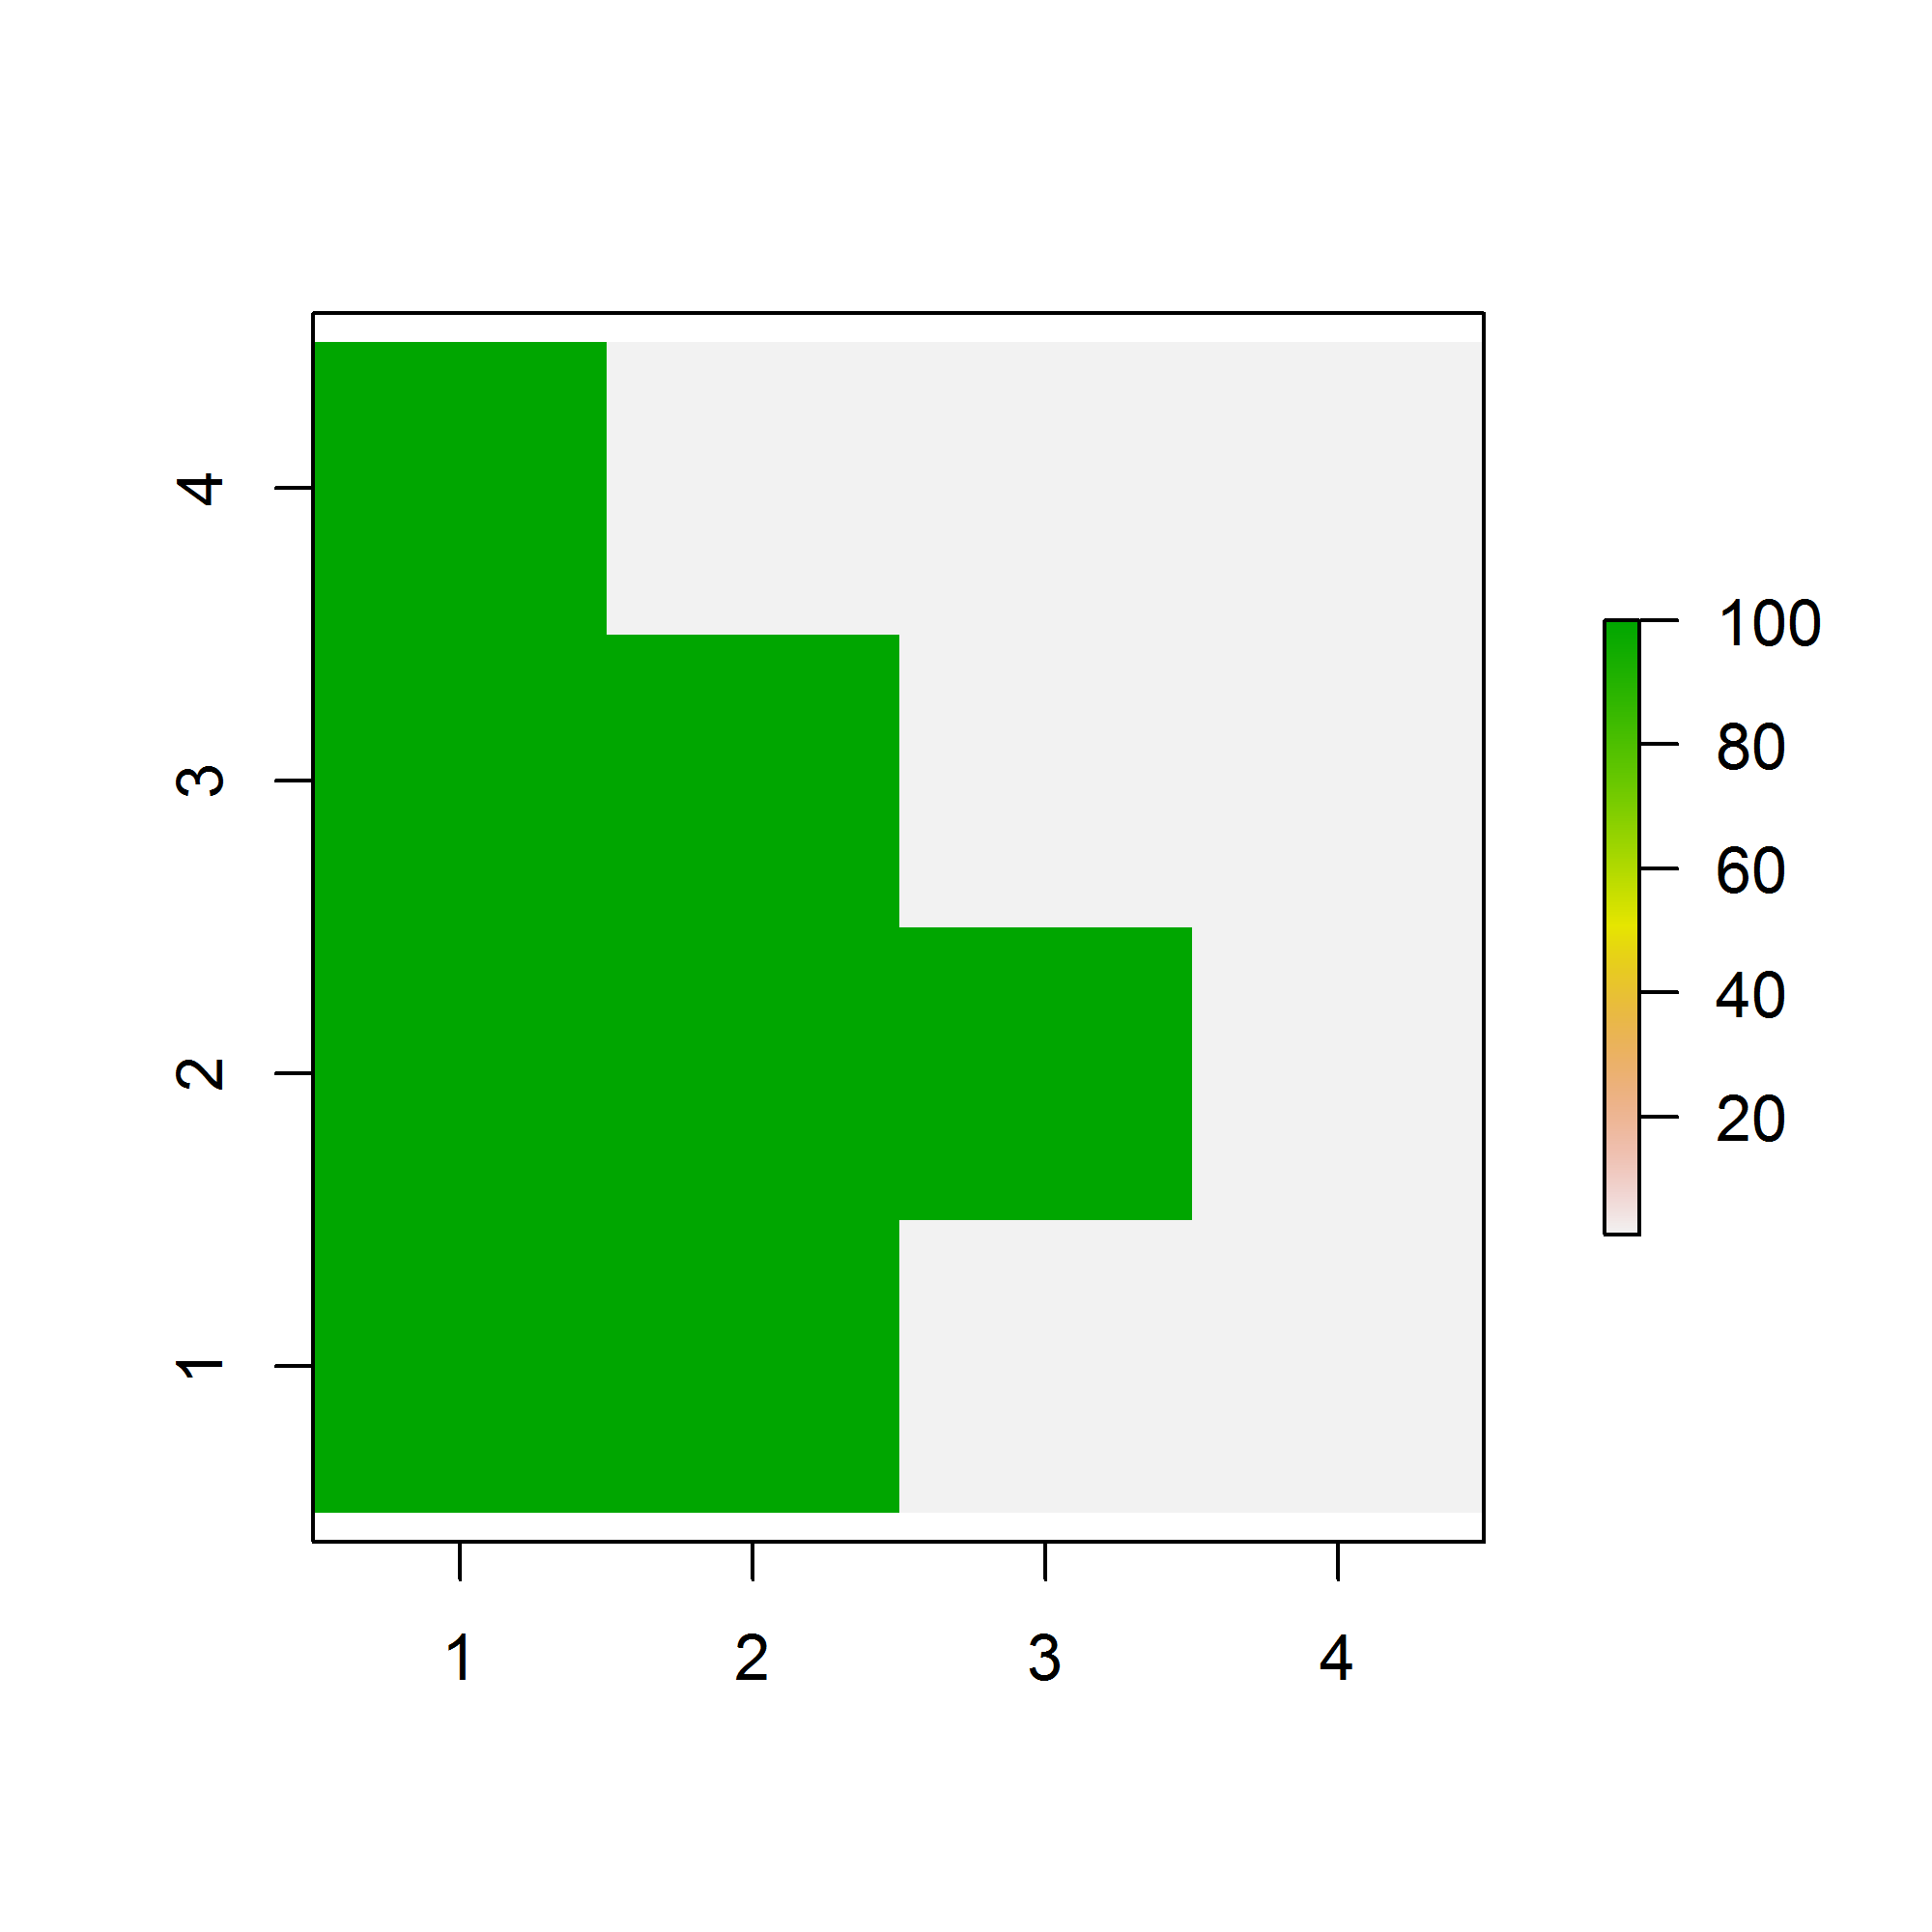
\includegraphics[height=3.25in,width=3.25in]{Ch10/figs/raster_2values}
\end{center}
\caption{A $4 \times 4$ raster with cost = 1 (white) or 100 (shaded) to represent ease of movement across a pixel.}
\label{ecoldist.fig.raster}
\end{figure}

Then we use the functions \mbox{\tt transition}, \mbox{\tt
  geoCorrection} (which doesn't really do anything if the coordinate system
  is UTM)
 and \mbox{\tt costDistance} to compute the distance
matrix. The transition function computes the cost of making a transition between
any two pixels, and it operates on the inverse-scale (''conductance'') and so the
\mbox{\tt transitionFunction} argument is given as $1/mean(x)$. 

To compute the cost distance we prescribe a set of points, or between
two sets of points (which is handy when one of the sets is of trap
locations, and the other is of individual activity centers).
To compute the distances for pixels in a raster, 
we use the center points of each raster.  The {\bf R}
 commands altogether are as follows:
{\small 
\begin{verbatim}
tr1<-transition(r,transitionFunction=function(x) 1/mean(x),directions=8)
tr1CorrC<-geoCorrection(tr1,type="c",multpl=FALSE,scl=FALSE)
pts<-cbind( sort(rep(1:4,4)),rep(4:1,4))
costs1<-costDistance(tr1CorrC,pts)
outD<-as.matrix(costs1)
\end{verbatim}
}
Now we can look at the result and see if it makes sense to us. Here we
print the first 5 columns of this distance matrix and illustration a
couple of examples of calculating the minimum cost-weighted distance
between points:
\begin{center}
{\small
\begin{verbatim}
> outD[1:5,1:5]
         1         2        3        4         5
1   0.0000 100.00000 200.0000 205.2426  50.50000
2 100.0000   0.00000 100.0000 200.0000  71.41778
3 200.0000 100.00000   0.0000 100.0000 171.41778
4 205.2426 200.00000 100.0000   0.0000 154.74264
5  50.5000  71.41778 171.4178 154.7426   0.00000
\end{verbatim}
} 
\end{center}
The interesting one is that between point 1 and 4. Note that simply
taking the shortest Euclidean distance, weighted by cost, produces a
cost-weighted distance of $100 \times 1$ to move from pixel 1 to pixel
2, and similarlly from 2 to 3 and 3 to 4, producing a total
cost-weighted distance of $300$. However, the actual {\it least-cost
  path} has cost-weighted distance $205.2426$. 
The shortest path has an individual moving from pixel 1 to 5, then 5
to 10, 10 to 15, 15 to 12, 12 to 8 and 8 to 4 which should add up to
$205.2426$.

\section{Fitting Models of Space Usage by MLE}
\label{ecoldist.sec.mle}

Throughout much of this book we rely on Bayesian analysis by MCMC mostly using 
{\bf BUGS}, but sometimes (as in Chapt. \ref{chapt.mcmc}) developing our own 
implementations. However, sometimes we prefer to use likelihood estimation, such as when
we can compare a set of models directly by likelihood either to do a
direct hypothesis test of a parameter, or tabulate a bunch of AIC values. It turns out, for this class
of models for space usage based on ecological distance, we actually prefer likelihood methods
not because they have any conceptual or methodological benefit, but simply because
they are more computationally efficient to implement \citep{royle_etal:2012ecol}.
So here we adopt our formulation of maximum likelihood estimation \citep{borchers_efford:2008} 
from Chapt. \ref{chapt.mle} 
for the class of models based on ecological distance. This is really just a straightforward
adaption of that.

We continue to work here with the binomial model:
\[
	y_{ij}| {\bf s}_{i} \sim \mbox{Bin}(K, p_{\theta}(d_{lcp}({\bf x}_{j},{\bf s}_{i};\theta_{2}); \theta_{0}, \theta_{1})
\]
where we have indicated the dependence of $p_{ij}$ on the parameters
${\bm \theta}$, and also $d_{lcp}$ which
itself depends on $\theta_{2}$, and the latent variable ${\bf s}$.
%The parameters
%${\bm \theta}$ include whatever parameters are involved in the
%cost-weighted distance function, i.e., at least $\theta_{2}$ from
%Eq. \ref{eq.cost}.
For the random effect we have ${\bf s}_{i} \sim  \mbox{Unif}({\cal
  S})$.
The joint distribution of the data for individual $i$ is the product
of $J$ binomial terms (i.e., contributions from each of $J$ traps):

\[
  [{\bf y}_{i} | {\bf s}_{i} , \theta] =
  \prod_{j=1}^{J} \mbox{Bin}(K, p_{\theta}({\bf x}_{j},{\bf s}_{i}) )
\]

{\flushleft This} assumes that encounter of individual $i$ in each
trap is independent of encounter in every other trap. Conditional on
${\bf s}_{i}$ this is reasonable in most applications in our view.
 The so-called marginal likelihood is computed by removing
${\bf s}_{i}$, by integration,  from the conditional-on-${\bf s}$
likelihood and regarding the {\it marginal} distribution of the data
as the likelihood. That
is, we compute:

\[
  [y|{\bm \theta}] =
\int_{{\cal S}}  [ {\bf y}_{i} |{\bf s}_{i},{\bm \theta}] g({\bf s}_{i}) d{\bf s}_{i}
\]

{\flushleft where}, under the uniformity assumption, we have
$g({\bf s}) = 1/||{\cal S}||$.
The joint likelihood for all $N$ individuals, assuming independence of
encounters among individuals, is the product of $N$ such terms:

\[
{\cal L}({\bm \theta} | {\bf y}_{1},{\bf y}_{2},\ldots, {\bf y}_{N}) = \prod_{i=1}^{N}
[{\bf y}_{i}|{\bm \theta}]
\]

The key operation for computing the likelihood is solving the
2-dimensional integration problem to remove ${\bf s}$, which we
resolve as we did previously in Chapt. \ref{chapt.mle}, using the
rectangular rule for integration, and averaging the integrand over a
fine mesh of points.
Therefore, 
the marginal pmf of ${\bf y}_{i}$, is
approximated by
\begin{equation}
         [{\bf y}_{i}|\theta] = \frac{1}{nG} \sum_{u=1}^{nG}  [ {\bf
            y}_{i} |{\bf s}_u, \theta]
\label{mle.eq.intlik}
\end{equation}

To deal with the fact that $N$ is unknown, there are two key issues
that need to be addressed.  First is that we don't observe the
``all-zero'' encounter histories (i.e., $y_{ij} = 0$ for all $j$)
corresponding to uncaptured individuals, so we have to make sure we
compute the probability for that all zero encounter history which we
do operationally by tacking a row of zeros onto the encounter history
matrix. We include the number of such all-zero encounter histories as
an unknown parameter of the model, which we label $n_{0}$.  In
addition, we have to be sure to include a combinatorial term to
account for the fact that of the $n$ observed individuals there are
${N \choose n}$ ways to realize a sample of size $n$. The
combinatorial term involves the unknown $n_{0}$ and thus it must be
included in the likelihood.

We wrote an {\bf R} function to evaluate the likelihood which we optimize
using the {\bf R} function \mbox{\tt nlm}.
The likelihood is given in the {\tt scrbook} package as the function
\mbox{\tt intlik3ed}. The help file 
provides an example of its usage and for simulating data.

To use this function the cost covariate $z(x)$ has to be of class 
\mbox{\tt RasterLayer} which requires packages \mbox{\tt sp} and
\mbox{\tt raster} to manipulate. 
The following is a stylized and more concise verstion of the actual
function, and we apply this in the following section.

{\small
\begin{verbatim}
intlik3ed<-function(start=NULL,y=y,K=NULL,X=traplocs,
distmet="ecol",covariate,theta2=NA){

nc<-covariate@ncols
nr<-covariate@nrows
Xl<-covariate@extent@xmin
Xu<-covariate@extent@xmax
Yl<-covariate@extent@ymin
Yu<-covariate@extent@ymax
### ASSUMES SQUARE RASTER -- NEED TO GENERALIZE THIS
delta<- (Xu-Xl)/nc
xg<-seq(Xl+delta/2,Xu-delta/2,delta) 
yg<-seq(Yl+delta/2,Yu-delta/2,delta) 
npix.x<-length(xg)
npix.y<-length(yg)
area<- (Xu-Xl)*(Yu-Yl)/((npix.x)*(npix.y))
G<-cbind(rep(xg,npix.y),sort(rep(yg,npix.x)))
nG<-nrow(G)

if(distmet=="euclid")
D<- e2dist(X,G)  
if(distmet=="ecol"){
if(is.na(theta2))
theta2<-exp(start[4])
cost<- exp(theta2*covariate)
tr1<-transition(cost,transitionFunction=function(x) 1/mean(x),directions=8)
tr1CorrC<-geoCorrection(tr1,type="c",multpl=FALSE,scl=FALSE)
D<-costDistance(tr1CorrC,X,G)
}

theta0<-start[1]; theta1<-start[2]; n0<-exp(start[3])

probcap<- (exp(theta0)/(1+exp(theta0)))*exp(-theta1*D*D)
Pm<-matrix(NA,nrow=nrow(probcap),ncol=ncol(probcap))
ymat<-y ; ymat<-rbind(y,rep(0,ncol(y)))
lik.marg<-rep(NA,nrow(ymat))
for(i in 1:nrow(ymat)){
Pm[1:length(Pm)]<- (dbinom(rep(ymat[i,],nG),rep(K,nG),probcap[1:length(Pm)],log=TRUE))
lik.cond<- exp(colSums(Pm))
lik.marg[i]<- sum( lik.cond*(1/nG) )  
}                                                 
nv<-c(rep(1,length(lik.marg)-1),n0)
part1<- lgamma(nrow(y)+n0+1) - lgamma(n0+1)
part2<- sum(nv*log(lik.marg))
out<-  -1*(part1+ part2)
out
}
\end{verbatim}
}

\subsection{Bayesian Analysis}

It is difficult to fit these models using the {\bf BUGS} engines
because it is not possible, to the best of our knowledge, to compute
the least-cost path distance.  It would be possible to fit the models
in {\bf BUGS} if the parameter $\theta_{2}$ was fixed. In that case,
one could compute the distance matrix ahead of time and reference the
required elements for a given ${\bf s}$.
Alternatively, it would be possible to write a custom MCMC routine
using the methods we present in Chapt. \ref{chapt.mcmc}, although we
have not yet developed our own implementation.




\section{Example: SCR model based on ecological distance}

In this section we provide examples that we think are typical of how
cost-weighted distance models can be used in real capture-recapture
problems.  We define a $20 \times 20$ pixel covariate raster with
extent = $[0.5, 4.5] \times [0.5, 4.5]$.  We regard this, for the
purposes of our example, as a coarse landscape covariate, with pixels
having some arbitrary scaling say, a $2 \times 2$ km resolution. Thus,
the raster defines a landscape of $40 \times 40$ km and we suppose
that 16 camera traps are established at the integer coordinates
$(1,1), (1,2), \ldots, (4,4)$. We could think of this as a landscape
within which we're studying a population of ocelots, lynx or some
other cat.

For our analyses, cost is characterized by a single covariate raster
and we consider two specific cases. First is an increasing trend from
the NW to the SE (''systematic raster''), where $z(x)$ is defined as
$z(x) = r(x) + c(x)$ where $r(x)$ and $c(x)$ are just the row and
column, respectively, of the raster.  This might define something
related to distance from an urban area or a gradient in habitat
quality due to land use, or environmental conditions such as
temperature or precipitation gradients.  In the second case we make up
a covariate by generating a field of spatially correlated noise to
emulate a typical patchy habitat covariate (''patchy raster'') such as
tree or understory density. The two covariates are shown in
Fig. \ref{ecoldist.fig.raster100}, along with a sample realization of
$N=100$ individuals (left panel only).  For both covariates we use a
cost function in which transitions from pixel ${\bf x}$ to ${\bf x}'$
is given by:

\[
 log(cost({\bf x},{\bf x}'))=  \theta_2 \frac{z({\bf x}) + z({\bf x}')}{2}
\]

{\flushleft where} $\theta_2 = 1$ for simulating the observed data.
 With $\theta_2=0$ then the
model reduces to one in which the cost of moving across each pixel is
constant, and therefore Euclidean distance is operative.

\begin{figure}
\begin{tabular}{cc}
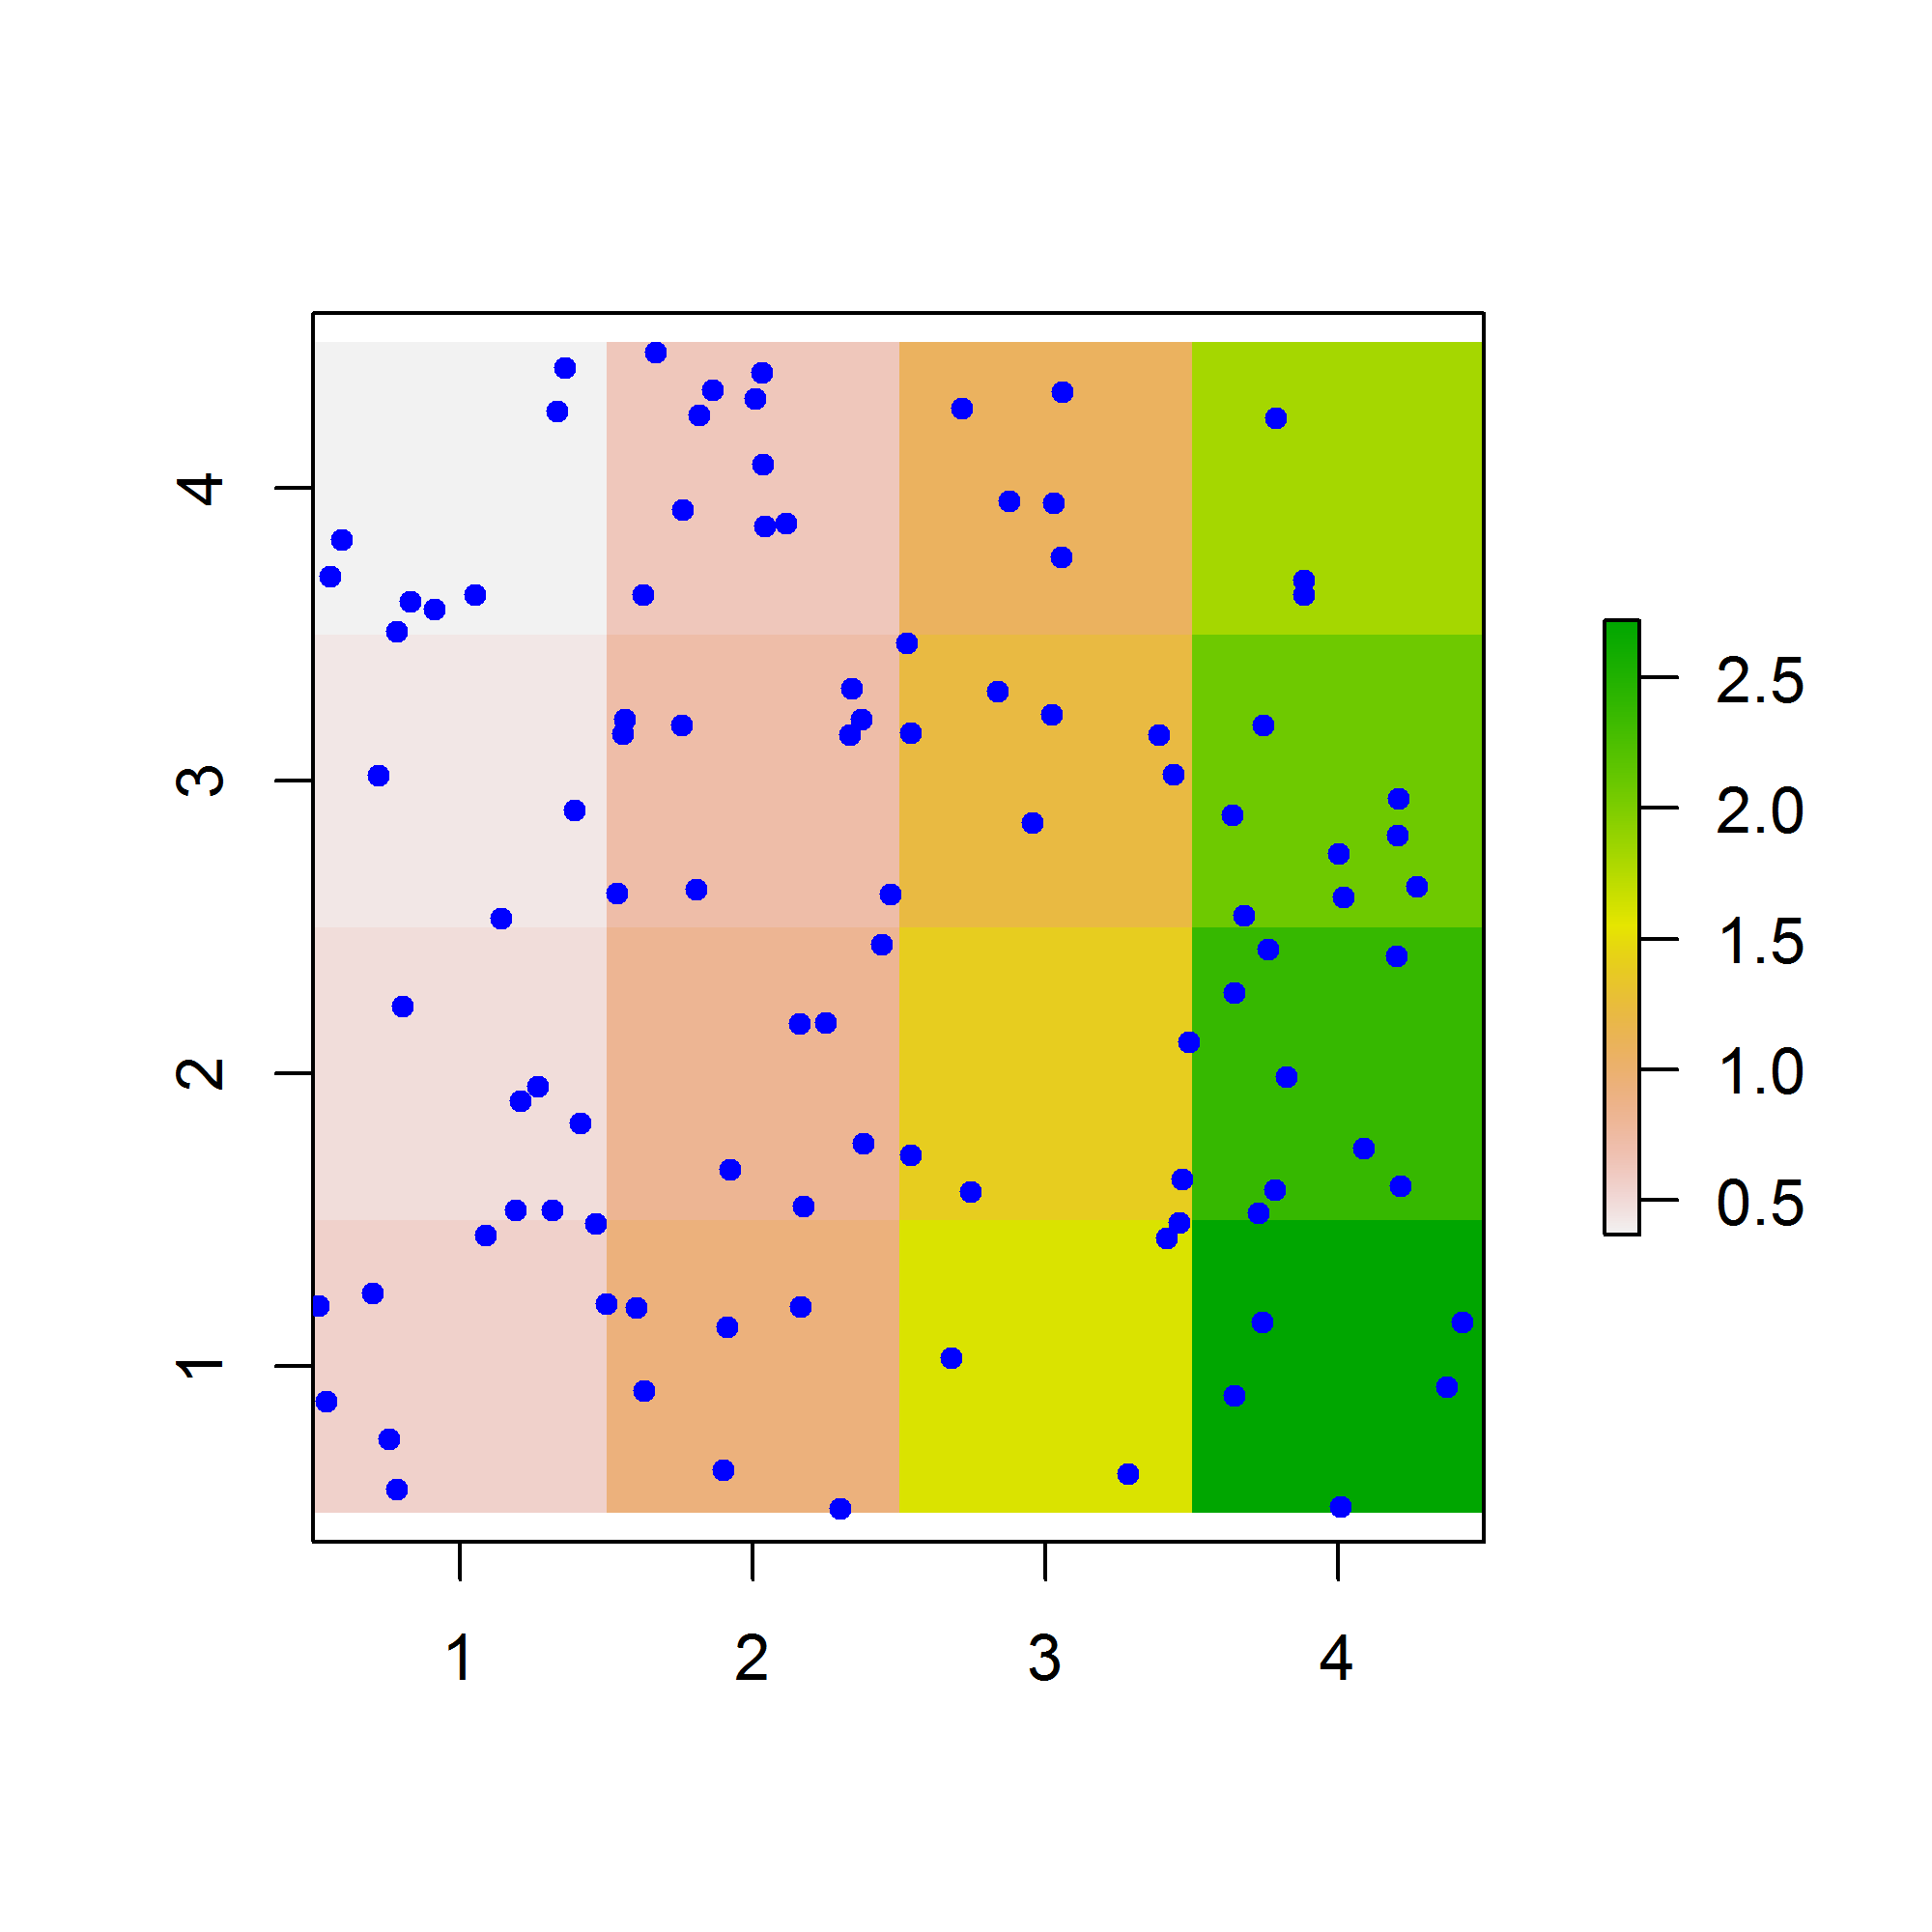
\includegraphics[height=3.25in,width=3.25in]{Ch10/figs/raster_withN100}
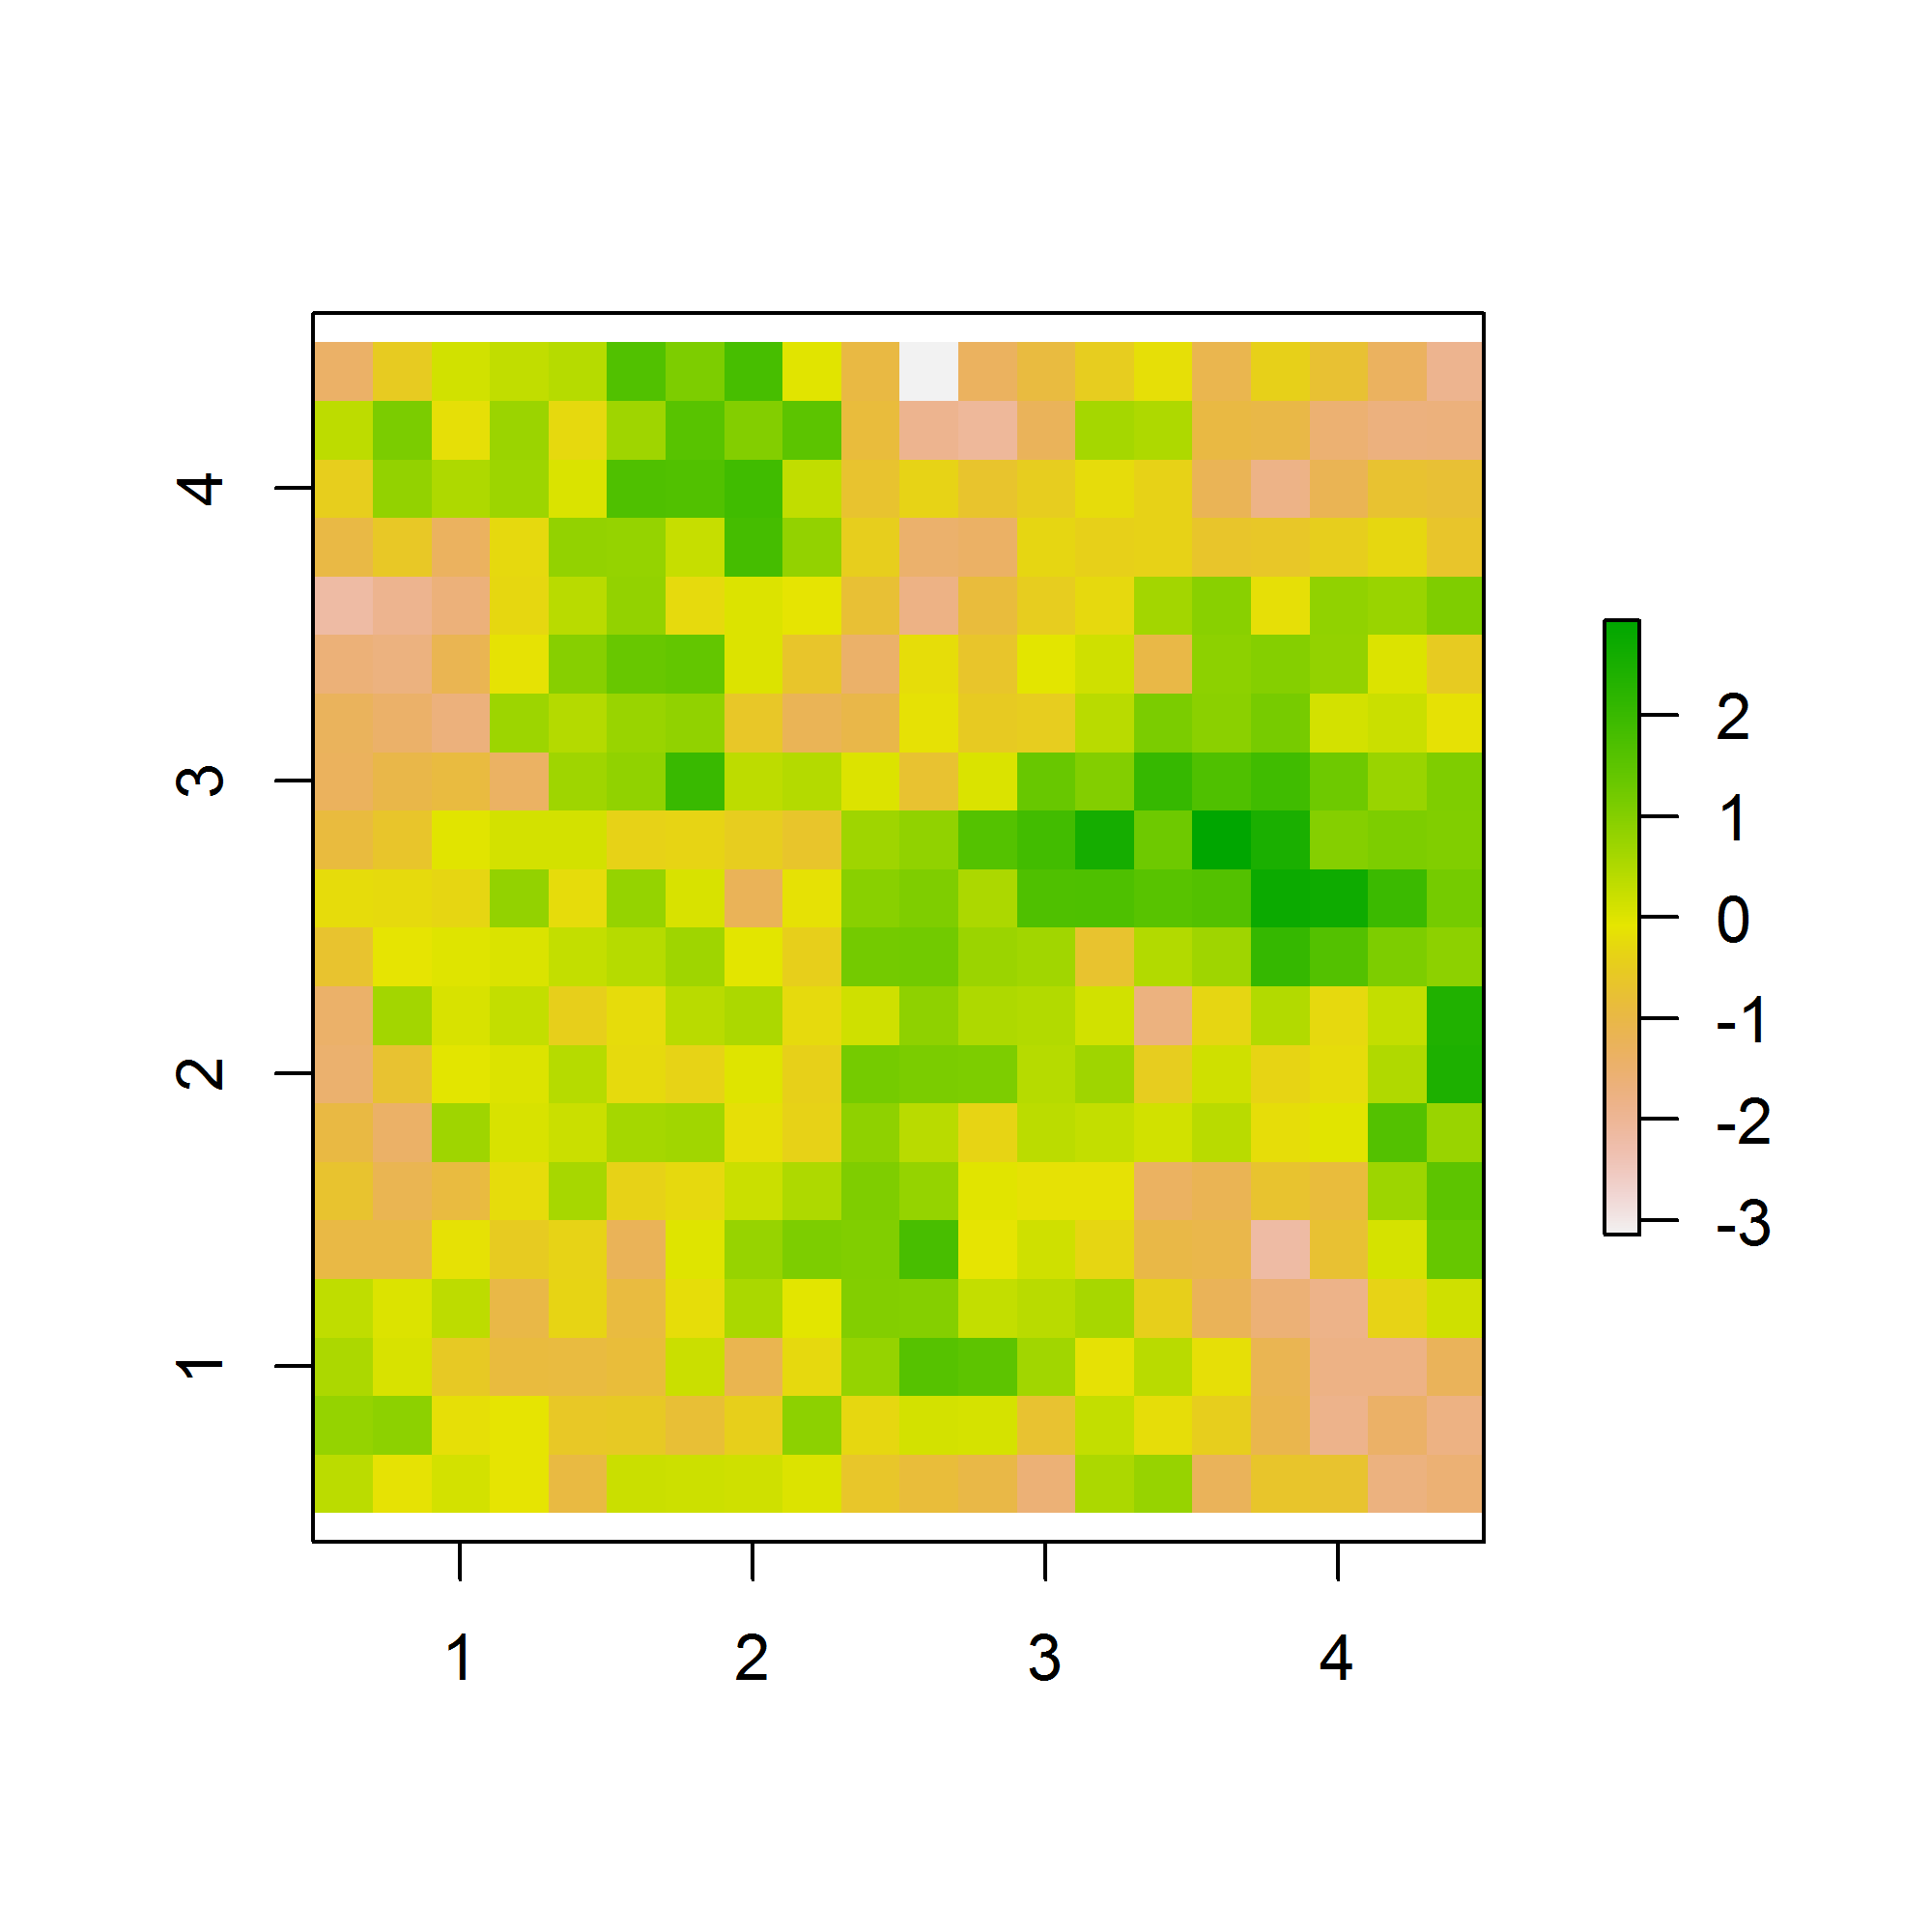
\includegraphics[height=3.25in,width=3.25in]{Ch10/figs/raster_krige} &
\end{tabular}
\caption{Two covariate rasters used for simulations. A hypothetical
  realization of $N=100$ activity centers is superimposed on the left,
along with 16 trap locations. }
\label{ecoldist.fig.raster100}
\end{figure}

\subsection{Non-stationarity of home range structure}

When distance is defined by the cost-weighted distance metric given
by Eq. \ref{eq.lcp} then individual space-usage varies
spatially in response to the landscape covariate(s) used in the
distance metric. For example, using one of the covariates we use in
our simulation study below (Fig. \ref{ecoldist.fig.raster100}, right
panel) with a Gaussian pdf detection function but having distance
metric defined by Eq. \ref{eq.lcp}, produces home ranges such
as those shown in Fig. \ref{fig.homeranges}. Later we simulate data
under the model that produces these home ranges and fit spatial
capture-recapture models to evaluate the efficacy of likelihood
estimation under this model.

\begin{figure}
\begin{center}
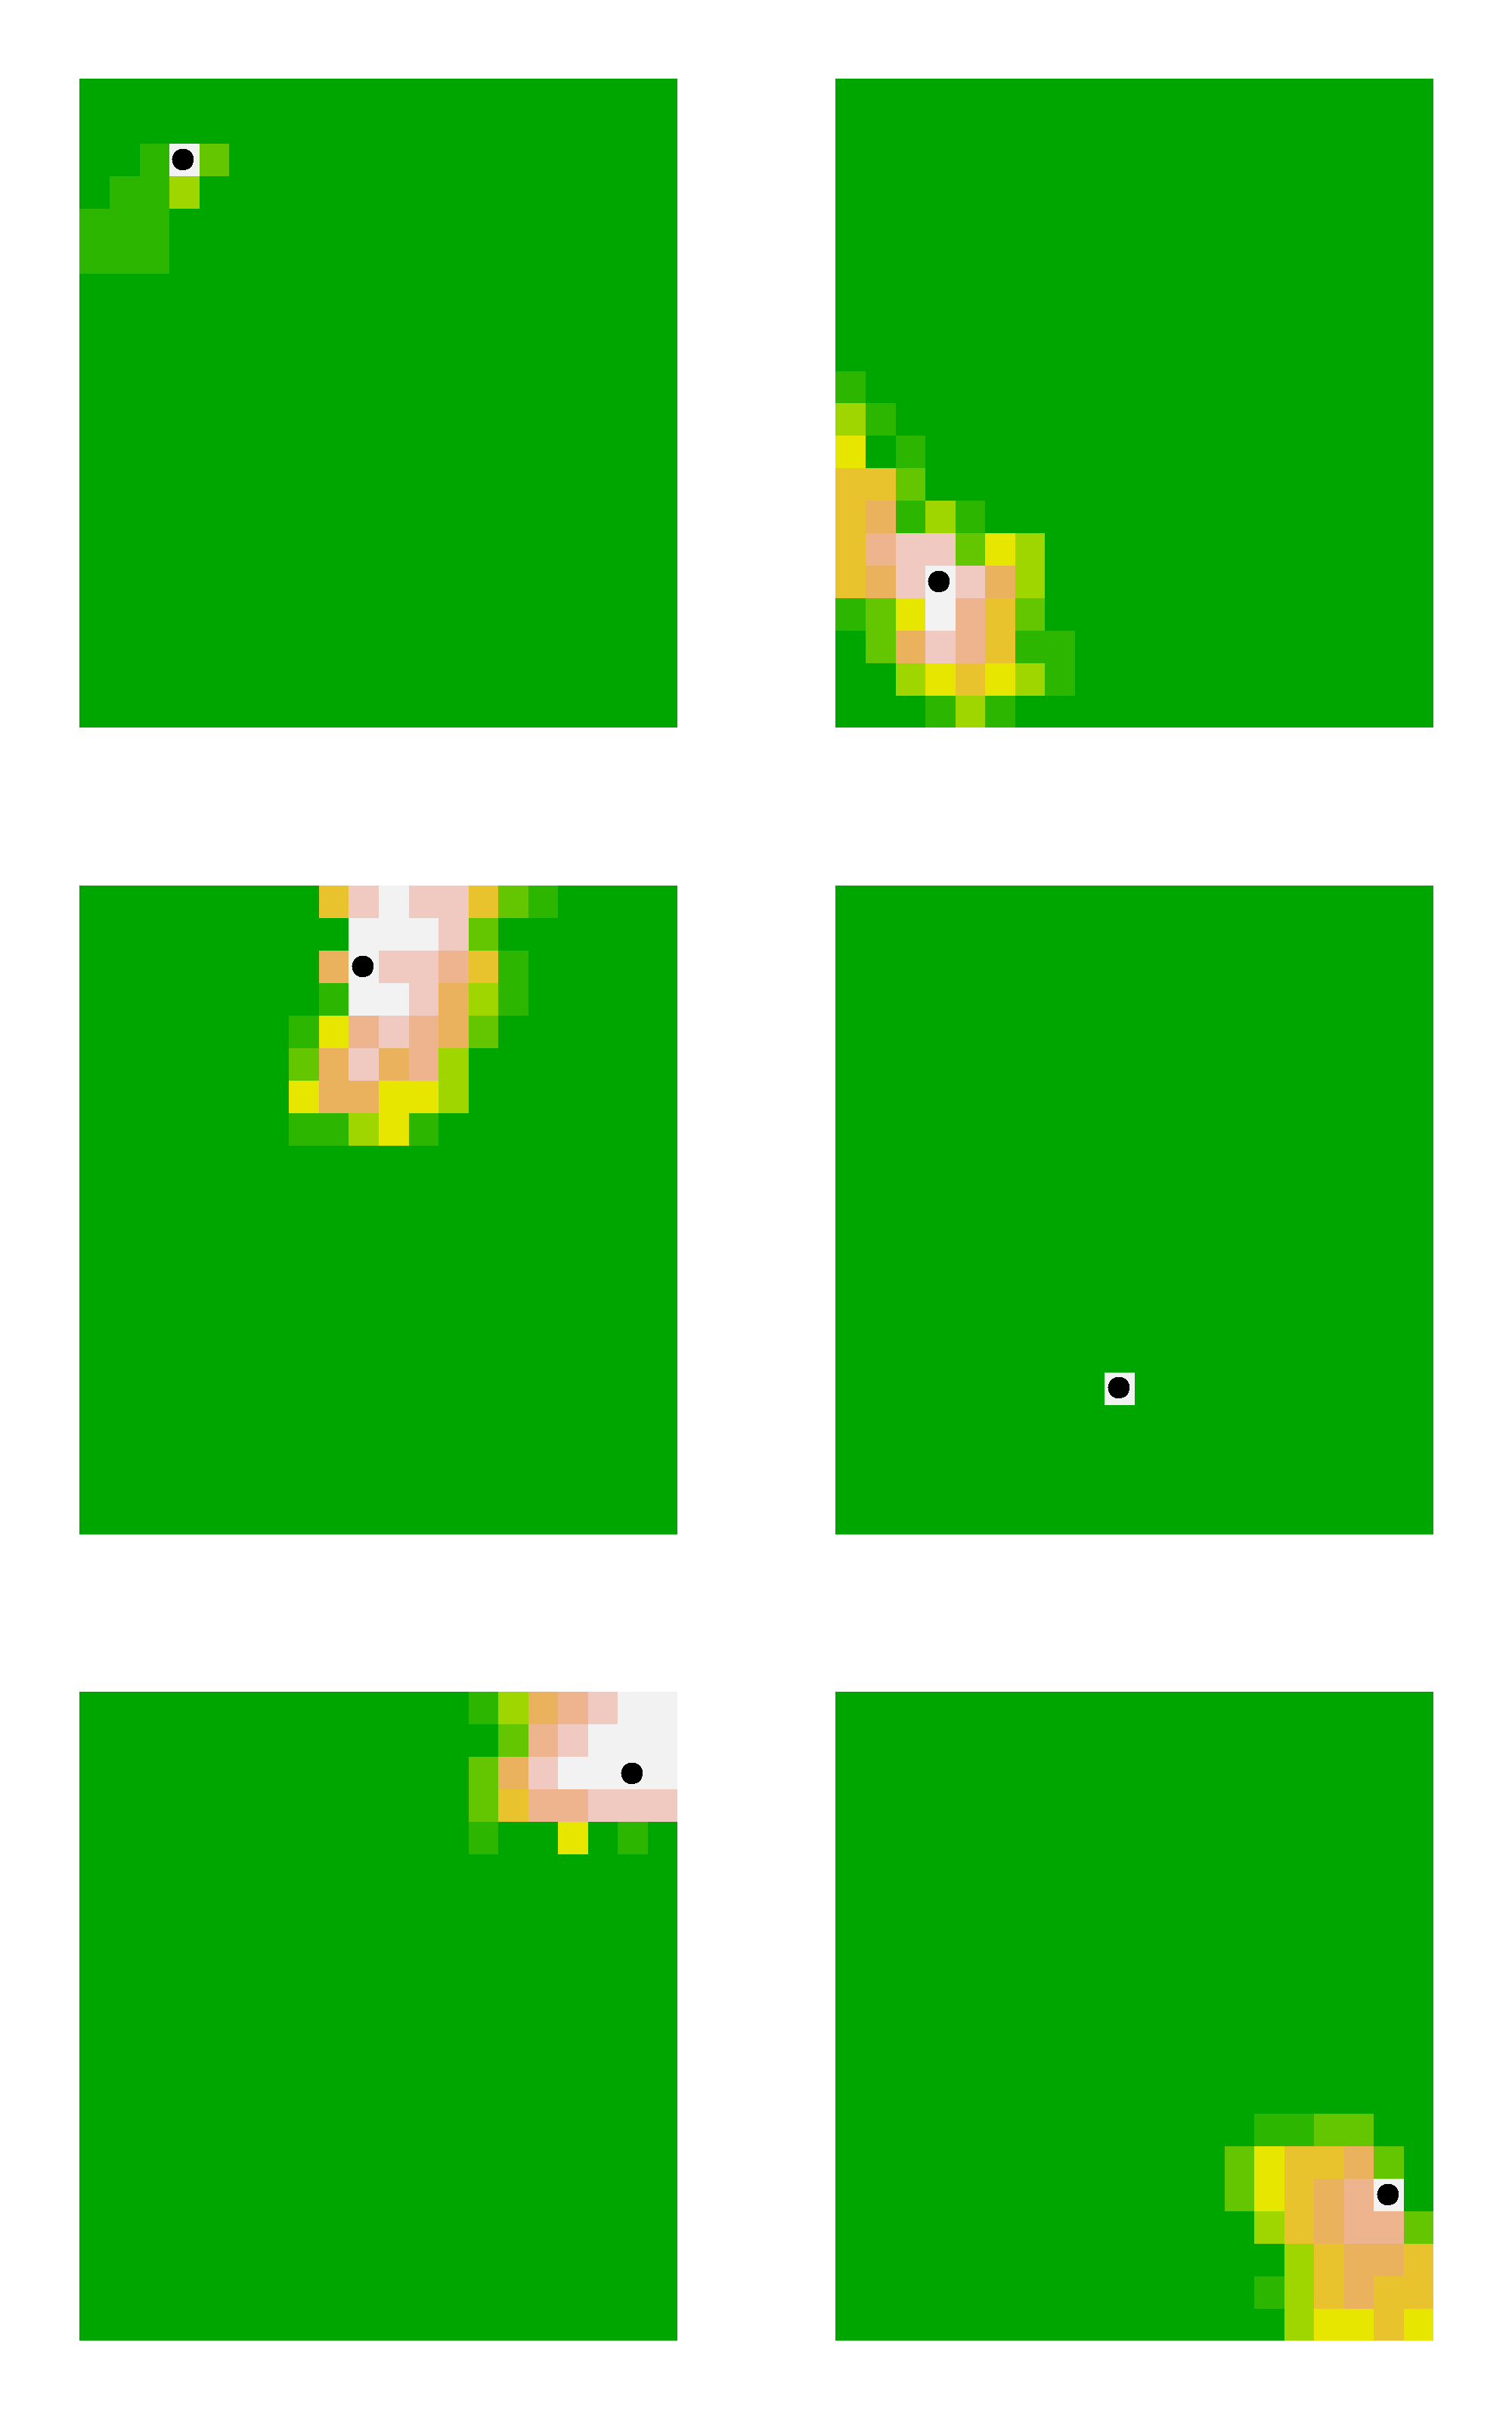
\includegraphics[height=6in,width=3.75in]{Ch10/figs/home_ranges}
\end{center}
\caption{
Typical home ranges for 6 individuals based on the cost surface shown in
  Fig. \ref{ecoldist.fig.raster100} with $\theta_{2}=1$. The black dot indicates the home
  range center and the pixels around each home range center are shaded
according to the probability of encounter, if a trap were located in
that pixel.
}
\label{fig.homeranges}
\end{figure}


\subsection{Simulation and Analysis}

We begin by simulating some data... we have to load the \mbox{\tt 
scrbook} library, use the function \mbox{\tt make.EDcovariates} to generate
our raster covariates, process that into a least-cost path distance
matrix, and then simulate observed encounter data using standard methods
which we have used many times previously in this book. The complete set
of {\bf R} commands is:

{\small 
\begin{verbatim}
library("scrbook")
out<-make.EDcovariates()
covariate<-out$covariate.patchy
set.seed(2013)

N<-200
theta0<- -2
sigma<- .5
K<- 5

theta1<- 1/(2*sigma*sigma)
r<-raster(nrows=20,ncols=20)
projection(r)<- "+proj=utm +zone=12 +datum=WGS84"
extent(r)<-c(.5,4.5,.5,4.5)
theta2<-1
cost<- exp(theta2*covariate)
tr1<-transition(cost,transitionFunction=function(x) 1/mean(x),directions=8)
tr1CorrC<-geoCorrection(tr1,type="c",multpl=FALSE,scl=FALSE)

# make up some trap locations
xg<-seq(1,4,1); yg<-4:1
pts<-cbind( sort(rep(xg,4)),rep(yg,4))

traplocs<-pts
points(traplocs,pch=20,col="red")
ntraps<-nrow(traplocs)

S<-cbind(runif(N,.5,4.5),runif(N,.5,4.5))
D<-costDistance(tr1CorrC,S,traplocs)
probcap<-plogis(theta0)*exp(-theta1*D*D)
# now generate the encounters of every individual in every trap
Y<-matrix(NA,nrow=N,ncol=ntraps)
for(i in 1:nrow(Y)){
 Y[i,]<-rbinom(ntraps,K,probcap[i,])
}
Y<-Y[apply(Y,1,sum)>0,]

\end{verbatim}
}


Now we use the {\bf R} function \mbox{\tt nlm} along with
our function to evaluate the likelihood and we can obtain the MLEs of the
model parameters. We'll do that for both the standard Euclidean distance
and then for the ecological distance based on the ``patchy'' covariate:
{\small
 \begin{verbatim}
frog1<-nlm(intlik3ed,c(theta0,theta1,3)),hessian=TRUE,y=Y,K=K,X=traplocs,
               distmet="euclid",covariate=covariate,theta2=1)

frog2<-nlm(intlik3ed,c(theta0,theta1,3,-.3),hessian=TRUE,y=Y,K=K,X=traplocs,
               distmet="ecol",covariate=covariate,theta2=NA)
\end{verbatim}
}

Show nlm() output for each and comment .......................XXXX

\subsection{Simulation study}

\citet{royle_etal:2012ecol}
carried-out a limited simulation study to evaluate the
general statistical performance of the density estimator under
this new model, the effect of mis-specifying the model with a
normal Euclidean distance metric and whether the parameter of the
cost function could be effectively estimated.
We recapitulate their results here. 
For population sizes of 100 and 200 individuals with activity
centers randomly distributed on the $20 \times 20$ landscape, they
subjected individuals
to encounter by 16 traps arranged in a $4\times 4$ grid 
using a Gaussian 
encounter model with least-cost path distance metric:
\[
log(p_{ij})= \theta_{0} + \theta_{1} d_{lcp}({\bf x}_{j},{\bf
  s}_{i}; \theta_{2})^{2}
\]
with  $\theta_{0} = -2$ and $\theta_{1} = 2$, the latter value
corresponding to $\sigma = 0.5$ of a stationary bivariate normal home
range model.  Different numbers of replicate samples were considered
$K=3,5,10$
(e.g., nights in a camera trapping study) in order
to produce varying sample
sizes. 

Three different models were fitted
to each simulated data set: the
misspecified euclidean distance model; (ii) the true data-generating
model with the relative cost raster {\it known} and (iii) the true
data-generating model but estimating the relative cost parameter by
maximum likelihood.  We used the ``systematic'' and ``patchy''
covariates defined previously.

\subsection{Simulation Results}

For both landscapes and all simulation conditions (levels of $K$ and
$N$) the average sample sizes of individuals captured are given in
Tab. \ref{tab.samplesize}.  The simulation results for estimating $N$
for the prescribed state-space are presented in Table
\ref{tab.results1} 2 below.  For the ``patchy'' landscape we see extreme
bias in estimates of $N$ when the Euclidean distance is used. There is
moderate small sample bias of 3-5\% in the MLE of $N$ using the
least-cost distance which becomes negligible as $K$ increases. For
$N=200$ the bias is on the order of 2\% for the lowest sample size
case ($K=3$) but negligible otherwise.  Interestingly, for the
landscape exhibiting systematic structure, there is a persistent bias
in the MLE of $N$ of 1-3\% even for the highest level of $K$. We were
initially surprised by this but, in fact, it is due to the fact that
the state-space is small relative to the extent of the trap grid and
sensitivity to a state-space that is too small is expected because the
support of the integrand is truncated. In the particular case of the
systematic landscape, we find that, in the NW corner of the raster
where cost of movement is low, individuals use large areas of space,
and the fitted model is under-stating the apparent
heterogeneity in encounter probability for the prescribed raster.  We
found that the issue is resolved when the traps are moved away from
the boundary (see Appendix 3).

The performance of estimating the cost parameter $\theta_{2}$ mirrors
the results for estimating $N$ for the prescribed state space. In the
patchy landscape where we don't expect a systematic gradient in space
usage around the edge of the state-space, we see
(Table \ref{tab.results2}) that $\theta_{2}$ is estimated with
diminishing bias as the sample size increases, but with persistent
bias due to truncation of the likelihood under the systematic
landscape which, as with the MLE of $N$, is resolved by moving the
traps away from the edge of the raster. Equivalently, in practice,
this could be resolved by expanding the raster away from the trap
locations so that all regions used by animals exposed to capture are
included in the state-space.



\begin{table}[htp]
\centering
\caption{
Expected sample sizes of captured individuals under each configuration of
$N$ (population size for the prescribed state-space) and $K$ (number of replicate samples).
}
\begin{tabular}{l|rrrr}
 & \multicolumn{2}{c}{Systematic} & \multicolumn{2}{c}{Patchy}  \\
    & N=100 &  N=200  &   N=100 &  N=200  \\ \hline
K=3 &  38.69 &   78.17  &   37.30 &   74.93  \\
K=5 &  51.10 &  103.18  &   51.89 &  103.71 \\
K=10&  65.81 &  132.39  &   69.44 &  138.76 \\
\end{tabular}
\label{tab.samplesize}
\end{table}


\begin{table}[htp]
\centering
\caption{
Mean of sampling distribution of the cost function parameter
$\theta_{2}$ for the different simulation
conditions. 
}
\begin{tabular}{l|rrrr}
 & \multicolumn{2}{c}{Patchy} & \multicolumn{2}{c}{Systematic} \\
    & N=100 &  N=200  &   N=100 &  N=200  \\ \hline
K=3 &   1.05&    1.03 &     1.17 & 1.14 \\
K=5 &   1.02&    1.01 &     1.12 &1.12 \\
K=10&   1.01&    1.00 &     1.10 &1.08 \\
\end{tabular}
\label{tab.results2}
\end{table}





\section{Illustration: Example Good vs. Bad habitat}

We provide another illustration of how to employ ecological distance
calculations in SCR models. This example shows more GIS-like analysis
for a situation where we have something like a hard habitat boundary
created to mimic a habitat corridor or park unit or some other block
of relatively homogeneous good-quality habitat for some species. This
particular system (shown in Fig. \ref{ecoldist.fig.corridor}), could
be habitat surrounded by a suburban wasteland of McDonalds and
Wal-Marts, much less hospital habitat for most species.  For our
purposes, we suppose that individuals live within the buffered ``f''
shaped region, although we could also imagine the negative of the
situation in which individuals live outside of the region, so that the
polygon represents a barrier (a lake) or bad habitat (an urban area)
or similar.  We describe the steps for creating this landscape
shortly, so that the reader can use a similar process to generate more
relevant landscapes for their own problems.

In this case we're not going to estimate any parameters of the cost
function (though we could) but instead we're going to use ecological
distance ideas only to constrain movement within (or to avoid)
landscape features.  However, the reader is encouraged to adapt the
likelihood function given in the previous section for this specific
case, so that a parameter of the cost function can be estimated.

\subsection{Basic Geographic Analysis in R}

In practical applications our landscape will contain one more more
polygons which delineate good or bad habitat or other important
characterisetics of the landscape.  These might exist as GIS
shapefiles or merely as a text file with coordinates defining polygon
boundaries. To work with polygons in the context of SCR models we need
to create a raster, overly the polygon and assign values to each pixel
depending on whether pixels are in the polygon or not, or how far they
are from polygon boundaries. These operations are relatively easy to
do within a GIS system but we need to be able to do them in ${\bf R}$
and we develop methods for this here.  See also
Chapts. \ref{chapt.mle} and \ref{chapt.mcmc} XXX exact sections ??
XXXX for examples of reading in the shapefile and using them to affect
calculations in SCR models.

The first thing we do here is create a set of polygons by
buffering and joining some line segments.
In the {\bf R} library \mbox{\tt scrbook}, we provide 
 a function \mbox{\tt make.seg} which allows the user to make such
 lines segments given a 
specific trap region.  To involve \mbox{\tt make.seg} we first
creating a plot region and then call \mbox{\tt make.seg} which has a
single argument being the number of points used to define the line
segment. In the following set of commands we generate two line
segments, \mbox{\tt l1} consisting of 9 points and \mbox{\tt l2}
consisting of 5 points, and these reside in a geographic region
enclosedd by $[0,10] \times [0,10]$:
{\small 
\begin{verbatim}
library("scrbook")
library("sp")
plot(NULL,xlim=c(0,10),ylim=c(0,10))
l1<-make.seg(9)
plot(l1)
l2<-make.seg(5)
plot(l1)
lines(l2)
\end{verbatim}
}

We used this function to create a couple of line segments of class
\mbox{\tt SpatialLines} from the {\bf R} package \mbox{\tt sp}, which
can be loaded from \mbox{\tt scrbook} as  follows
\begin{verbatim}
data("fakecorridor")
\end{verbatim}
This has 2 line files in it (\mbox{\tt l1} and \mbox{\tt l2}) and a
trap locations file (\mbox{\tt traps}). 
We use some functions from the {\bf R} packages \mbox{\tt sp} and
\mbox{\tt rgeos} to join and 
buffer (by 0.5 units) the two segments. The commands are as follows
and the result is shown in Fig. \ref{ecoldist.fig.corridor}.

{\small
\begin{verbatim}
data("fakecorridor")
library("sp")
library("rgeos")

buffer<- 0.5
par(mfrow=c(1,1))
aa<-gUnion(l1,l2)
plot(gBuffer(aa,width=buffer),xlim=c(0,10),ylim=c(0,10))
pg<-gBuffer(aa,width=buffer)
pg.coords<- pg@polygons[[1]]@Polygons[[1]]@coords

xg<-seq(0,10,,40)
yg<-seq(10,0,,40)

delta<-mean(diff(xg))
pts<- cbind(sort(rep(xg,40)),rep(yg,40))
points(pts,pch=20)

in.pts<-point.in.polygon(pts[,1],pts[,2],pg.coords[,1],pg.coords[,2])
points(pts[in.pts==1,],pch=20,col="red")
\end{verbatim}
}

\begin{figure}
\begin{center}
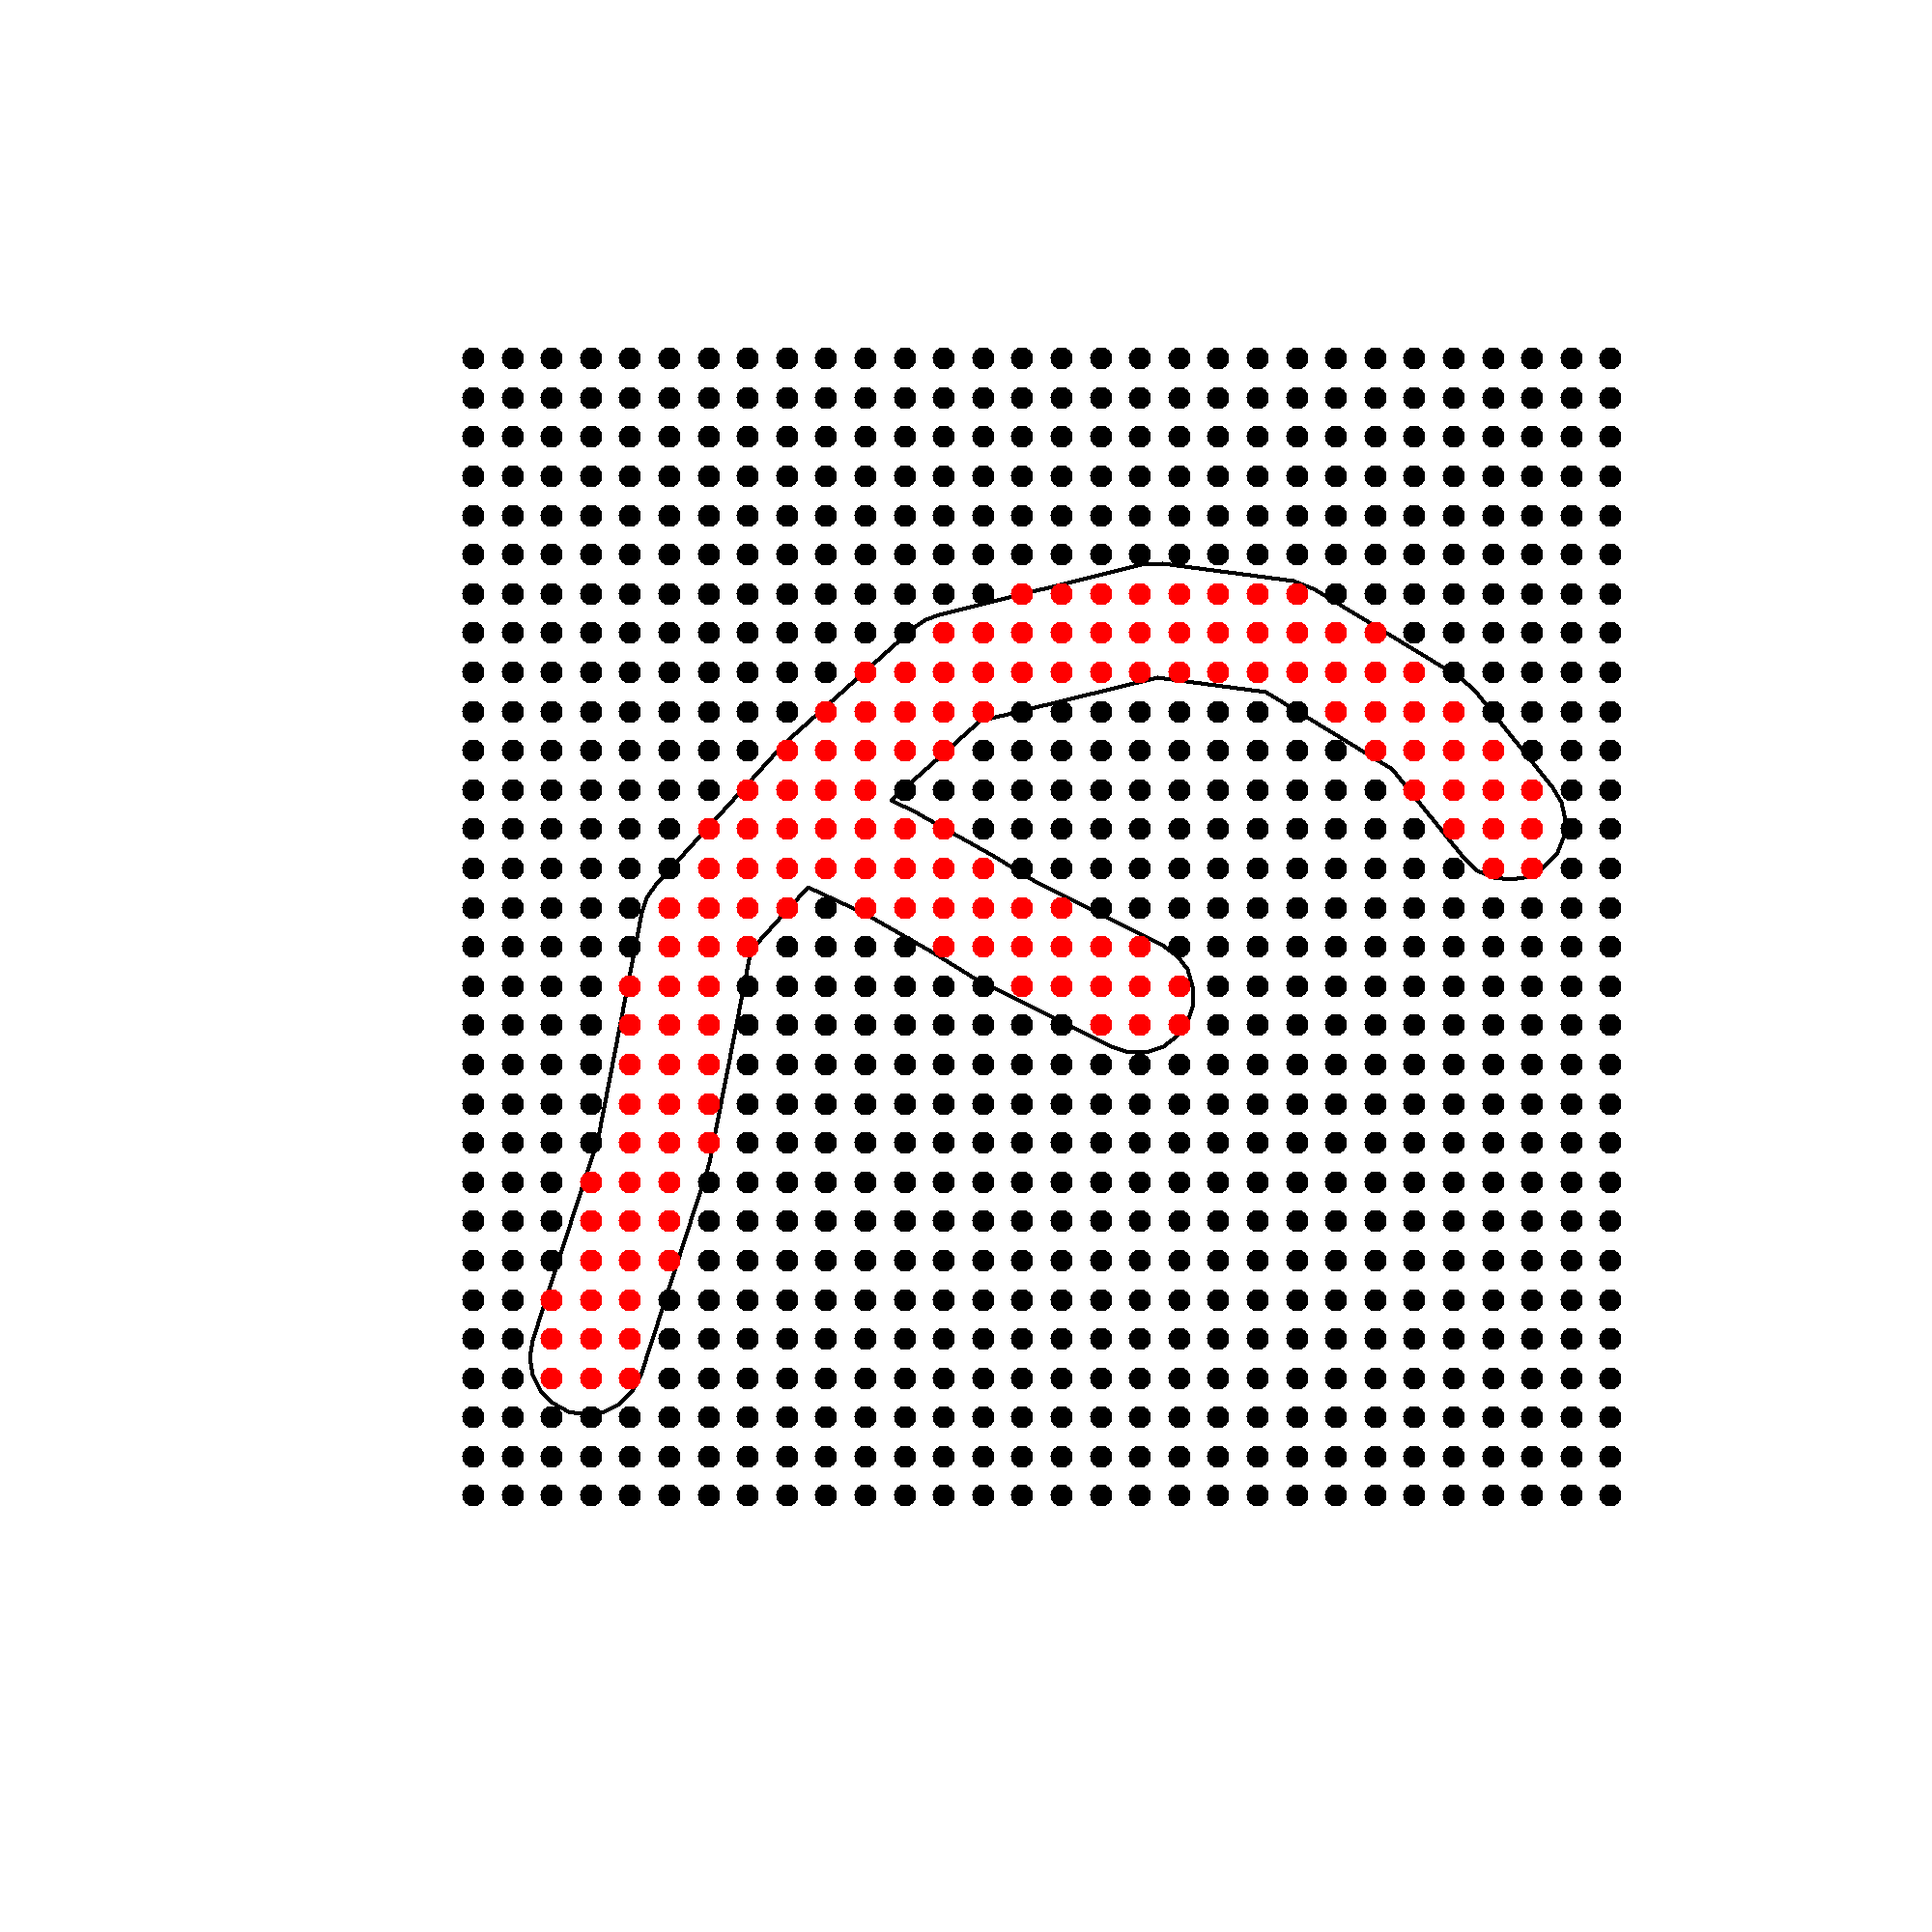
\includegraphics[height=3.25in,width=3.25in]{Ch10/figs/corridor}
\end{center}
\caption{A made-up corridor or reserve.}
\label{ecoldist.fig.corridor}
\end{figure}


We focus on devising a SCR model for this corridor system and we
imagine that animals will tend to severely avoid leaving the buffered
habitat zone. Therefore, we assign $\mbox{\tt cost}=1$ if a pixel 
is within the buffer,
and $\mbox{\tt cost} = 10000$ if a pixel is outside of a
buffer. Therefore the cost to move to a neighboring pixel outside of
the buffered area is $5000.5$ compared to the cost of 1 to move to a
neighboring pixel inside the buffer. 

In this example, we're not going to estimate parameters of the cost
function. Therefore, in that case, we can compute the ecological
distance matrix one time and modify our likelihood code to accept the
distance matrix as input. We give that likelihood in the library
\mbox{\tt scrbook} as the function \mbox{\tt intlik3edv2}.
We note also that it provides a vector of 0's and 1's that
define any potential state-space restrictions. In the analysis of this
simulated data set, we define the state-space to be the buffered
corridor system. The help file for \mbox{\tt intlik3edv2} contains the
script that follows.

In this case we simulate N=200 guys in the corridor system and so we
restrict out state-space accordingly for purposes of fitting the
model. However we encourage the reader to refit the model without the
state-space restriction (for fitting the model only) and then
contemplate the result.  The code for doing all of this is as follows

{\small 
\begin{verbatim}
cost<-rep(NA,nrow(pts))
cost[in.pts==1]<-1      # low cost to move among pixels but not 0
cost[in.pts!=1]<-10000  # high cost 

library("raster")
r<-raster(nrows=40,ncols=40)
projection(r)<- "+proj=utm +zone=12 +datum=WGS84"
extent(r)<-c(0-delta/2,10+delta/2,0-delta/2,10+delta/2)
values(r)<-matrix(cost,40,40,byrow=FALSE)
par(mfrow=c(1,1))
plot(r)
points(pts,pch=20,cex=.4)

library("gdistance")
tr1<-transition(r,transitionFunction=function(x) 1/mean(x),directions=8)
tr1CorrC<-geoCorrection(tr1,type="c",multpl=FALSE,scl=FALSE)
costs1<-costDistance(tr1CorrC,pts)
outD<-as.matrix(costs1)
plot(pts,pch=".")
points(pts[in.pts==1,],pch=20,col="red")

library(``scrbook'')
traplocs<-traps$loc
trap.id<-traps$locid
ntraps<-nrow(traplocs)

set.seed(2013)
N<-200
S.possible<- (1:nrow(pts))[in.pts==1]
S.id<-sample(S.possible,N,replace=TRUE)
S<- pts[S.id,]

D<- outD[S.id,trap.id]
eD<- e2dist(S,traplocs)
Dtraps<-outD[trap.id,]

alpha0<- -1.5
sigma<- 1.5
beta<- 1/(2*sigma*sigma)
K<-10

probcap<-plogis(alpha0)*exp(-beta*D*D)
Y<-matrix(NA,nrow=N,ncol=ntraps)
for(i in 1:nrow(Y)){
 Y[i,]<-rbinom(ntraps,K,probcap[i,])
}
Y<-Y[apply(Y,1,sum)>0,]

frog1<-nlm(intlik3edv2,c(-2.5,2,log(4)),hessian=TRUE,y=Y,K=K,X=traplocs,
            S=pts,D=Dtraps,inpoly=in.pts)
frog2<-nlm(intlik3edv2,c(-2.5,2,log(4)),hessian=TRUE,y=Y,K=K,X=traplocs,
            S=pts,D=Deuclid,inpoly=in.pts)
\end{verbatim}
}

In the example that we ran abovve we compared the result for using
distance-within-the-corridor to normal Euclidean distance and the
results do not differ too much in this single instance. 


\section{A stream network}

Later we might add a 3rd prototype situation involving a stream network. 

We could use ``distance from stream'' to model effects of habitat
and corridors or whatever


\section{Summary and Outlook}


All published applications of SCR models to date have been based on models for the
encounter probability that are functions of the standard Euclidean
distance between individuals and traps. The obvious limitations are
that it is unaffected by landscape or habitat structure and implies
stationary, isotropic and symmetrical home ranges. These are standard
criticisms of the basic SCR model as universally applied in
practice. However, it is not a relevant criticism of the basic
conceptual formulation of SCR models, because, as we have
demonstrated, one can modify the Euclidean distance metric to
accommodate more realistic space usage considerations.  Following
\citet{royle_etal:2012ecol},
we demonstrated how to use 
minimum cost-weighted distance (i.e., ``least-cost
path'') between points, and where ``cost'' is characterized by one or
more spatially explicit covariates that are believed to influence
movement or space-usage of individuals. 

How animals use space and therefore how distance to a trap is
perceived by individuals is not something that can ever be known. We
can only ever conjure up models to describe this phenomenon and fit
those models to limited data on a sample of individuals during a
limited amount of time.  Here we have shown that there is hope to
estimate parameters, from capture-recapture data, that describe how
animals use space and thereby allow for irregular home range geometry
that is influenced by landscape structure.

Not surprisingly, our simulation study demonstrated
(Table 2) that the MLE of model parameters is
approximately unbiased in moderate sample sizes. Moreover, the effect
of ignoring ecological distance and using normal Euclidean distance in
the model for encounter probability, has the logical effect of causing
negative bias in estimates of $N$.  We expect this because the effect
is similar to failing to model heterogeneity. i.e., if we mis-specify
``model $M_h$'' \citep{otis_etal:1978} with ``Model $M_0$''
\citep{otis_etal:1978} then we will expect to under-estimate $N$. So
the effect of mis-specifying the ecological distance metric with a
standard homogeneous Euclidean distance has the same effect. As a
practical matter, it stands to reason that many previous applications
of SCR models based on homogeneous distance metrics have under-stated
density of the focal population.

In our view, this bias is not really the most important reason to
consider models of ecological distance. Rather, inference about the
structure of ecological distance is fundamental to many problems in
applied and theoretical ecology related to modeling landscape
connectivity, corridor and reserve design, population viability
analysis, gene flow, and other phenomena.  Our new model allows
investigators to evaluate landscape factors that influence movement of
individuals over the landscape from non-invasively collected
capture-recapture data.  Therefore SCR models based on ecological
distance metrics might aid in corridor design and understanding other
aspects of space usage and movement in animal populations.

We considered inference for ecological distance models based on 
marginal likelihood \citep{borchers_efford:2008}
(see Chapt. \ref{chapt.mle}).
In principle,
Bayesian analysis does not pose any unique challenges for this new
class of models, except that computing the cost-weighted distance is
computationally intensive.  So, having to do this at each iteration of
an MCMC algorithm may be impractical using existing algorithms.  A
related issue is that the size of the raster slows things down. For
very large rasters, even likelihood analysis can be computationally
challenging and methods for efficient calculation of the ecological
distance given the raster covariate(s) and parameters might be needed.



\begin{table}[h!]
\label{tab.results1}
{\small
\caption{Simulation results for estimating population size $N$ for a prescribed state-space with
$N=100$ or $N=200$ and various levels of replication ($K$) chosen to affect the observed sample
size of individuals (Tab. \ref{tab.samplesize}). For each simulated data set, the SCR model was fitted with
standard Euclidean distance (``euclid''), least-cost path assuming the
cost parameter $\theta_2$ is known (``lcp/known''), or allowing it to
be estimated by maximum likelihood (``lcp/est'').
The summary statistics of the
sampling distribution reported are the mean, standard deviation
(``SD'') and quantiles (0.025, 0.50, 0.975).
}
{\bf Systematic trend raster:} \\
\begin{tabular}{l|rrrrr|rrrrr}
         & \multicolumn{5}{c}{N=100   } & \multicolumn{5}{c}{N=200  }  \\
         &   mean &  SD  & 0.025 & 0.50 & 0.975  & mean  & SD   & 0.025 & 0.50  & 0.975 \\ \hline
K=3      &        &      &       &      &        &       &      &       &       &       \\
euclid   &   63.65& 12.62& 44.77 & 61.17&  90.98 & 126.68& 17.05&  98.93& 124.49& 168.26 \\
lcp/known&   99.28& 20.80& 68.83 & 97.55& 152.59 & 196.47& 27.39& 152.03& 192.96& 259.78\\
lcp/est  &  101.93& 21.68& 67.95 &101.56& 156.21 & 201.58& 28.14& 154.96& 200.15& 263.20\\
K=5      &        &      &       &      &        &       &      &       &       &        \\
euclid   &  64.60 & 7.11 & 51.52 & 63.86&  77.33 & 130.02& 10.25& 113.48& 128.96& 151.32\\
lcp/known&  95.96 &11.64 & 74.21 & 96.16& 117.65 & 193.04& 17.13& 166.84& 191.88& 226.16\\
lcp/est  &  98.94 &12.97 & 74.68 & 99.00& 123.88 & 198.80& 19.60& 166.87& 197.97& 239.46\\
K=10     &        &      &       &      &        &       &      &       &       &       \\
euclid   &  69.24 & 4.83 & 59.37 & 69.47&  79.18 & 139.83&  7.62& 125.65& 139.65& 154.82\\
lcp/known&  94.46 & 7.04 & 81.45 & 94.04& 108.83 & 190.47& 11.55& 170.49& 189.74& 213.19\\
lcp/est  &  97.53 & 8.18 & 82.02 & 97.62& 113.16 & 195.19& 13.28& 171.63& 194.58& 217.96\\ \hline
\end{tabular}
\\
{\bf Patchy "random" raster: } \\
\begin{tabular}{l|rrrrrrrrrr}
         & \multicolumn{5}{c}{N=100  } & \multicolumn{5}{c}{N=200   }  \\
         &   mean &  SD  & 0.025 & 0.50  & 0.975  & mean  & SD   & 0.025 & 0.50  & 0.975 \\ \hline
K=3      &        &      &       &       &        &       &      &       &       &       \\
euclid   &  78.68 & 18.12& 49.40 & 76.34 & 125.47 & 154.34& 33.74& 107.00& 146.34& 221.43\\
lcp/known& 109.09 & 27.52& 69.50 &104.86 & 183.72 & 207.18& 46.53& 143.31& 198.42& 315.89\\
lcp/est  & 110.96 & 28.65& 69.55 &106.98 & 181.84 & 208.77& 49.29& 141.68& 197.89& 325.77\\
K=5      &        &      &       &       &        &       &      &       &       &        \\
euclid   &  77.85 & 11.55& 59.17 & 77.44 & 101.14 & 153.39& 15.57& 129.31& 149.54& 185.38\\
lcp/known& 103.57 & 15.83& 78.15 &100.58 & 137.48 & 201.57& 21.25& 165.94& 199.95& 243.26\\
lcp/est  & 104.44 & 15.79& 78.38 &101.47 & 139.55 & 200.91& 20.78& 164.42& 200.47& 246.46\\
K=10     &        &      &       &       &        &       &      &       &       &       \\
euclid   &  78.01 & 5.26 & 68.00 & 77.96 & 87.81  & 156.27&  8.51& 142.17& 156.05& 174.55\\
lcp/known&  99.84 & 7.09 & 86.86 & 99.84 & 114.11 & 198.64& 11.04& 181.43& 197.62& 220.45\\
lcp/est  & 100.42 & 7.56 & 86.72 &100.34 & 115.47 & 198.45& 11.44& 180.06& 198.04& 219.52\\ \hline
\end{tabular}
}
\end{table}







\newpage







\begin{table}[ht]
{\small
\caption{Simulation results for estimating population size $N$ for a prescribed state-space with
$N=100$ or $N=200$ and various levels of replication ($K$) chosen to affect the observed sample
size of individuals. These results correspond to those of the
systematic landscape in Table 2 except with the traps
moved 0.5 units in from the boundary of the raster.
Each grouping of 3 rows (for a given value of $K$) summarizes the
performance of $\hat{N}$ under 3 distance models: (1) A model in which
Euclidean distance was used (``euclid''); (2) A model in which the
least-cost path distance was used, with the coefficient of the cost
function fixed (``lcp/known''); and (3) A model in which the
coefficient was estimated (``lcp/est''). The summary statistics of the
sampling distribution reported are the mean, standard deviation
(``SD'') and quantiles (0.025, 0.50, 0.975).
}
{\bf Systematic trend raster:} \\
\begin{tabular}{l|rrrrr|rrrrr}
         & \multicolumn{5}{c}{N=100   } & \multicolumn{5}{c}{N=200  }  \\
         &   mean &  SD  & 0.025 & 0.50 & 0.975  & mean  & SD   & 0.025 & 0.50  & 0.975 \\ \hline
K=3      &        &      &       &      &        &       &      &       &       &       \\
euclid   &   84.48& 20.42& 51.16 & 81.51& 140.62 &163.70 &24.55 &126.64 &157.67 &223.63 \\
lcp/known&  104.14& 25.49& 65.67 &101.50& 173.19 &200.16 &29.27 &158.65 &191.04 &268.78\\
lcp/est  &  105.90& 26.19& 65.95 &103.40& 182.30 &201.34 &29.54 &161.88 &192.36 &268.98\\
K=5      &        &      &       &      &        &       &      &       &       &       \\
euclid   & 81.21  &11.33 &61.35  &79.20 & 98.86  &163.27 &13.06 &140.21 &162.97 &185.94\\
lcp/known& 99.93  &12.86 &76.97  &99.75 &117.76  &199.80 &16.60 &170.25 &198.23 &227.66\\
lcp/est  & 100.84 &13.15 &79.96  &99.51 &119.08  &200.25 &16.53 &168.88 &199.29 &227.39\\
K=10     &        &      &       &      &        &       &      &       &       &       \\
euclid   &  80.10 & 7.81 &66.45  &79.14 &93.33   &158.40 & 9.25 &142.74 &157.86 &173.18\\
lcp/known& 100.07 & 9.50 &82.99  &100.33&114.81  &197.62 &12.58 &171.95 &199.21 &217.19\\
lcp/est  & 100.10 & 9.88 &82.31  &100.91&116.27  &197.52 &13.03 &169.49 &200.68 &217.82\\ \hline
\end{tabular}
}
\label{tab.results3}
\end{table}





















